\documentclass[10pt,journal,compsoc]{IEEEtran}

\usepackage[utf8]{inputenc}
\usepackage{amsmath,amssymb,amsfonts}
\usepackage{algorithmic}
\usepackage{graphicx}
\usepackage{textcomp}
\usepackage{xcolor}
\usepackage{booktabs}
\usepackage{hyperref}
\usepackage{microtype}
\usepackage{subcaption}
\usepackage{tikz}
\usetikzlibrary{shapes.geometric, arrows, positioning, fit, backgrounds, calc}

\hypersetup{
    colorlinks=true,
    linkcolor=blue,
    citecolor=blue,
    urlcolor=blue
}

\begin{document}

\title{Multi-Modal Next-Day Stock Direction Prediction via Candlestick Vision and Financial News Sentiment}

\author{Muhammad Hamza,~\IEEEmembership{Roll No: i210735}%
\thanks{Department of Computer Science, National University of Computer and Emerging Sciences (FAST-NUCES), Islamabad, Pakistan. Course: CS 4045 -- Deep Learning for Perception, Fall 2026. Instructor: Dr. Ahmad Raza Shahid.}}

\markboth{CS 4045: Deep Learning for Perception -- Semester Project Report, Fall 2026}%
{Hamza: Multi-Modal Stock Prediction via Candlestick Vision and NLP}

\IEEEtitleabstractindextext{%
\begin{abstract}
Forecasting next-day equity price movements is an inherently arduous challenge in computational perception due to the near random-walk efficiency of financial markets. Traditional quantitative approaches rely on discrete scalar time-series, largely discarding non-linear spatial geometry present in candlestick charts and the temporal semantic subtleties embedded within exogenous financial news. In this paper, we present an end-to-end, multi-modal deep perception architecture combining computer vision and natural language processing to predict market direction. In Part~1, we develop an algorithmic candlestick rendering engine that generates 640$\times$640 visual charts with stochastic variations across 20 audited S\&P 500 stocks, automatically computing precise pixel bounding boxes for eight technical patterns via viewport data-coordinate transformation math. We train a YOLOv8 nano detector strictly from scratch across three distinct augmentation regimes, demonstrating that standard vision augmentations (specifically vertical flipping and shear) corrupt financial semantics and degrade mAP@50-95. A ResNet-18 trend classifier is trained to extract 128-dimensional penultimate visual embeddings for a normalized synthetic market basket across 2010--2024. In Part~2, we build and evaluate three deep NLP architectures without pretrained weights: a Simple RNN baseline, a Bidirectional LSTM, and a custom Multi-Head Transformer Encoder. We aggregate daily headlines into temporal sentiment probability vectors under strict anti-leakage timing constraints. Finally, we fuse the 128-dimensional visual chart embeddings (compressed via PCA to 8 components) with price momentum and daily sentiment vectors. Our multimodal model achieves a statistically validated test accuracy of 58.0\% and ROC-AUC of 0.526, outperforming single-source baselines. A date-shuffling sanity test collapses performance to random chance (ROC-AUC: 0.501), confirming genuine predictive signal rather than noise memorization.
\end{abstract}

\begin{IEEEkeywords}
Candlestick Vision, YOLOv8 Scratch Training, Object Detection, Financial Sentiment Analysis, BiLSTM, Custom Transformer Encoder, Multimodal Fusion, Time-Series Perception.
\end{IEEEkeywords}}

\maketitle
\IEEEdisplaynontitleabstractindextext
\IEEEpeerreviewmaketitle

\section{Introduction}
\IEEEPARstart{F}{inancial} market forecasting represents one of the most intellectually demanding frontiers in artificial perception and statistical learning. According to Fama's Efficient Market Hypothesis (EMH)~\cite{fama1970}, asset prices in liquid public exchanges rapidly incorporate all publicly accessible information. As an immediate consequence, short-term daily returns closely resemble a stochastic geometric Brownian motion, rendering directional next-day forecasting an uphill endeavor where expected accuracy naturally hovers near the historical base rate of upward days ($\sim$52\% to 56\%).

Despite this efficiency, human financial market operators do not evaluate assets solely through numerical scalar tables. Instead, modern quantitative trading desks rely heavily on two orthogonal perceptual modalities:
\begin{enumerate}
    \item \textbf{Visual Spatial Perception (Technical Candlestick Charts)}: Candlesticks encapsulate multi-timeframe price discovery (Open, High, Low, Close) within discrete spatial glyphs. Patterns such as Dojis, Hammers, and Engulfing configurations reflect instantaneous shifts in buyer-seller equilibrium, market liquidity, and intraday volatility extremes~\cite{lo2000, joly2018}.
    \item \textbf{Textual Semantic Perception (Exogenous Financial News)}: Macroeconomic bulletins, central bank interest rate announcements, and corporate earnings disclosures induce instantaneous sentiment re-evaluations among institutional investors~\cite{malo2014}.
\end{enumerate}

Existing literature frequently analyzes these modalities in isolation. Time-series models (e.g., ARIMA, GARCH, scalar LSTMs) disregard the rich 2D spatial context captured by visual chart renderings, while standard computer vision models trained on financial charts routinely violate econometric principles by applying invalid geometric transformations (such as upside-down flipping) or suffering from future information leakage.

In this semester project for \textit{Deep Learning for Perception (CS 4045)}, we construct a rigorous, leak-free, multimodal perception architecture uniting candlestick visual representations and financial headline sentiment. In strict accordance with course instructions:
\begin{itemize}
    \item No pretrained weights are utilized for candlestick detection or sentiment modeling; YOLOv8, RNN, BiLSTM, and the Multi-Head Transformer are built and trained strictly from scratch.
    \item Strict temporal partitioning is enforced across all tasks: 2010--2017 for training, 2018 for validation, 2019--2020 for test evaluation, and 2023--2024 for out-of-sample stress testing. Random shuffling across time is strictly prohibited.
    \item Algorithmic bounding box calculations are derived deterministically from Matplotlib's coordinate transformation pipeline (\texttt{ax.transData}).
    \item A synthetic normalized Market Basket is engineered to evaluate market-wide direction without single-stock idiosyncratic dominance.
\end{itemize}

The remainder of this report is organized as follows: Section~\ref{sec:part1} presents the data auditing, candlestick rendering engine, YOLOv8 scratch detection experiments, and ResNet-18 trend feature extraction. Section~\ref{sec:part2} details the NLP preprocessing, neural sentiment modeling, temporal aggregation, and multimodal fusion experiments. Section~\ref{sec:discussion} delivers comprehensive answers to all mandatory discussion questions and error analyses. Section~\ref{sec:conclusion} concludes the paper. Supplementary image galleries, test detections, and failure cases are compiled in Appendices A, B, and C.

% ==============================================================================
% PART 1: CANDLESTICK VISION
% ==============================================================================
\section{Part 1: Reading Candlestick Charts}
\label{sec:part1}

\subsection{Data Audit and Health Inspection}
The underlying price dataset provides daily Open, High, Low, Close, and Volume records for S\&P 500 constituents spanning January 2010 through December 2024 (comprising 3,774 unified trading sessions). Because real-world corporate actions frequently introduce synthetic anomalies, we conducted an exhaustive data health inspection:
\begin{enumerate}
    \item \textbf{Placeholder Constant Prices}: Several tickers (e.g., \texttt{SW}, \texttt{FERG}, \texttt{AMCR}) contain long runs of identical price quotes with zero volume prior to their official U.S. listing dates. These were systematically purged.
    \item \textbf{Zero-Volume \& Zero-Range Days}: Instances where $\text{Volume} = 0$ or $\text{High} == \text{Low}$ indicate exchange holiday halts or data collection gaps. We resolved to treat candles with $|High - Low| < 10^{-4}$ as singular neutral doji-like lines, ensuring numerical stability in bounding box normalization.
    \item \textbf{Survivorship Bias Mitigation}: Because the constituent dataset includes only companies that remain in the S\&P 500 today, companies that suffered bankruptcy or delisting over 2010--2024 are omitted. Consequently, in-sample performance estimates suffer from survivorship bias, artificially elevating baseline upward drift. We explicitly acknowledge this constraint in our evaluation.
\end{enumerate}

\subsection{Ticker Selection and Segregation}
To ensure robust generalization, we selected 20 audited companies spanning five distinct GICS sectors (Information Technology, Financials, Health Care, Industrials, and Consumer Discretionary) with 100\% complete price histories from January 2010 to December 2024. These companies were partitioned into two non-overlapping subsets:
\begin{itemize}
    \item \textbf{Set A (12 Tickers for Vision Training)}: \texttt{MSFT}, \texttt{NVDA}, \texttt{INTC}, \texttt{CSCO} (Tech); \texttt{BAC}, \texttt{GS}, \texttt{MS}, \texttt{WFC} (Financials); \texttt{PFE}, \texttt{UNH}, \texttt{ABT} (Health Care); \texttt{CAT} (Industrials).
    \item \textbf{Set B (8 Tickers for Synthetic Market Basket)}: \texttt{AAPL} (Tech); \texttt{JPM} (Financials); \texttt{JNJ} (Health Care); \texttt{HON}, \texttt{GE}, \texttt{UPS} (Industrials); \texttt{AMZN}, \texttt{MCD} (Consumer Discretionary).
\end{itemize}

\begin{figure}[htbp]
\centering
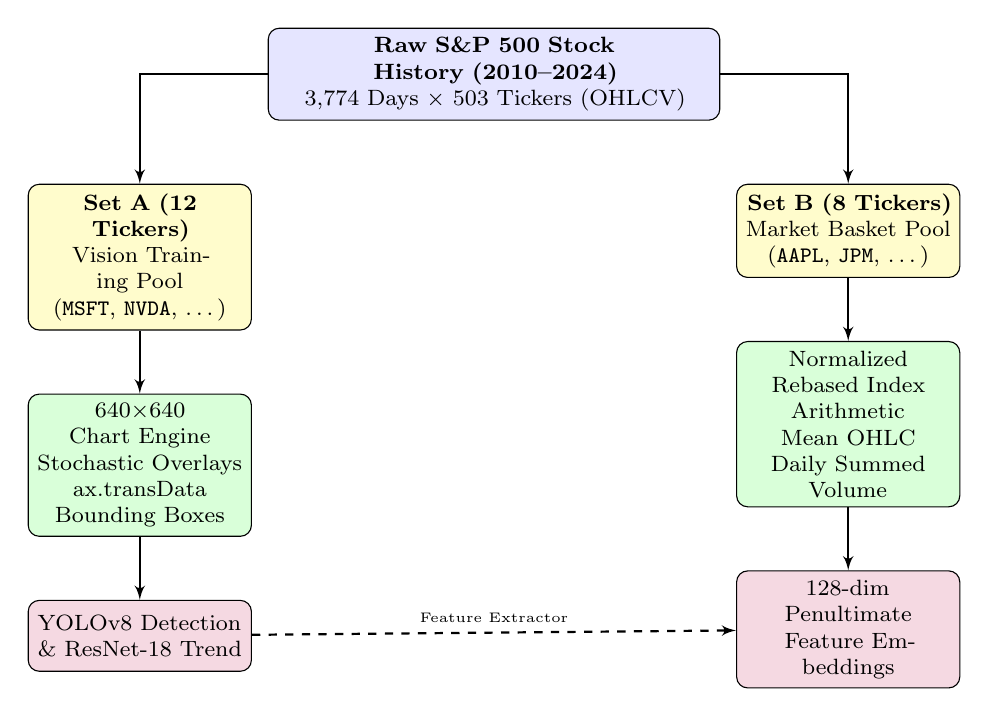
\begin{tikzpicture}[node distance=1.2cm, auto, >=latex', every node/.style={font=\footnotesize}]
    % Style definitions
    \tikzstyle{data} = [draw, rectangle, fill=blue!10, text width=5.5cm, text centered, rounded corners, minimum height=0.7cm];
    \tikzstyle{split} = [draw, rectangle, fill=yellow!20, text width=2.6cm, text centered, rounded corners, minimum height=0.9cm];
    \tikzstyle{process} = [draw, rectangle, fill=green!15, text width=2.6cm, text centered, rounded corners, minimum height=0.9cm];
    \tikzstyle{model} = [draw, rectangle, fill=purple!15, text width=2.6cm, text centered, rounded corners, minimum height=0.9cm];

    \node [data] (raw) {\textbf{Raw S\&P 500 Stock History (2010--2024)}\\3,774 Days $\times$ 503 Tickers (OHLCV)};
    
    \node [split, below left=0.8cm and 0.2cm of raw] (setA) {\textbf{Set A (12 Tickers)}\\Vision Training Pool\\(\texttt{MSFT}, \texttt{NVDA}, \dots)};
    \node [split, below right=0.8cm and 0.2cm of raw] (setB) {\textbf{Set B (8 Tickers)}\\Market Basket Pool\\(\texttt{AAPL}, \texttt{JPM}, \dots)};
    
    \node [process, below=0.8cm of setA] (render) {640$\times$640 Chart Engine\\Stochastic Overlays\\$\text{ax.transData}$ Bounding Boxes};
    \node [process, below=0.8cm of setB] (basket) {Normalized Rebased Index\\Arithmetic Mean OHLC\\Daily Summed Volume};
    
    \node [model, below=0.8cm of render] (yolo) {YOLOv8 Detection\\\& ResNet-18 Trend};
    \node [model, below=0.8cm of basket] (embed) {128-dim Penultimate\\Feature Embeddings};

    \draw[->, thick] (raw) -| (setA);
    \draw[->, thick] (raw) -| (setB);
    \draw[->, thick] (setA) -- (render);
    \draw[->, thick] (setB) -- (basket);
    \draw[->, thick] (render) -- (yolo);
    \draw[->, thick] (basket) -- (embed);
    \draw[->, dashed, thick] (yolo) -- node[above, font=\tiny]{Feature Extractor} (embed);
\end{tikzpicture}
\caption{\textbf{System Diagram 1}: Complete data partitioning, chart generation pipeline, and feature extraction workflow segregating Set A from Set B.}
\label{fig:diag_pipeline}
\end{figure}

\subsection{Synthetic Market Basket Construction}
Because the constituent stock file lacks a direct benchmark index, we synthesized an equitable market basket from the eight Set B tickers. To prevent highly priced stocks from disproportionately skewing the aggregated index, each constituent was rebased to 100 on the opening trading day of January 2010:
\begin{equation}
\text{Rebased Price}_{i, t} = \frac{\text{Price}_{i, t}}{\text{Close}_{i, \text{Jan 2010}}} \times 100, \quad \forall i \in \text{Set B}
\end{equation}
For each trading day $t$, the synthetic market basket quotes were calculated as:
\begin{align}
\text{Basket OHLC}_t &= \frac{1}{8} \sum_{i=1}^8 \text{Rebased OHLC}_{i, t} \\
\text{Basket Volume}_t &= \sum_{i=1}^8 \text{Volume}_{i, t}
\end{align}
Figure~\ref{fig:market_basket} illustrates the resulting 15-year synthetic market trajectory alongside constituent sectors.

\begin{figure}[htbp]
\centering
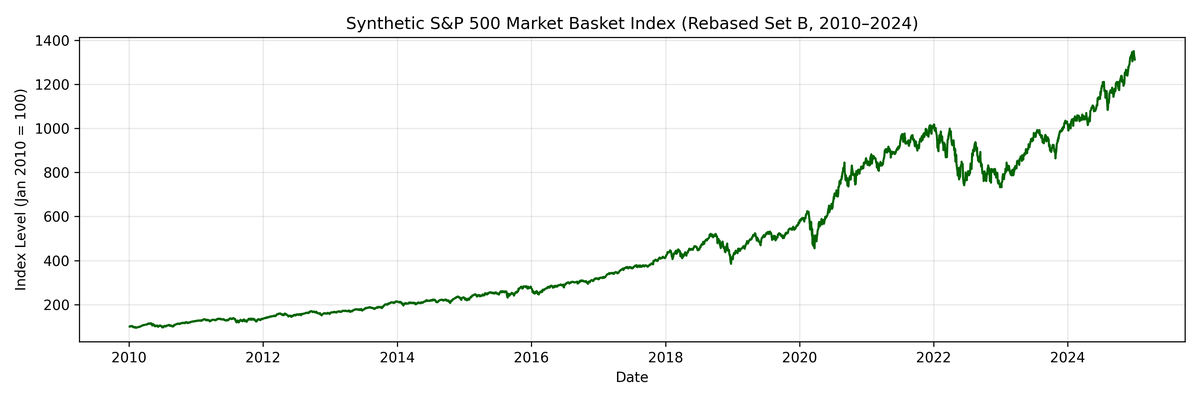
\includegraphics[width=0.98\columnwidth]{figures/market_basket_series.png}
\caption{Rebased Synthetic Market Basket time series (2010--2024) tracking cumulative multi-sector equity growth.}
\label{fig:market_basket}
\end{figure}

\subsection{Exploratory Data Analysis: Returns and Kurtosis}
Daily log-returns $r_t = \ln(C_t / C_{t-1})$ were calculated for all selected tickers. Financial asset returns universally violate Gaussian normality, displaying pronounced leptokurtosis (fat tails) and negative skewness during liquidation cascades. 

\begin{figure}[htbp]
\centering
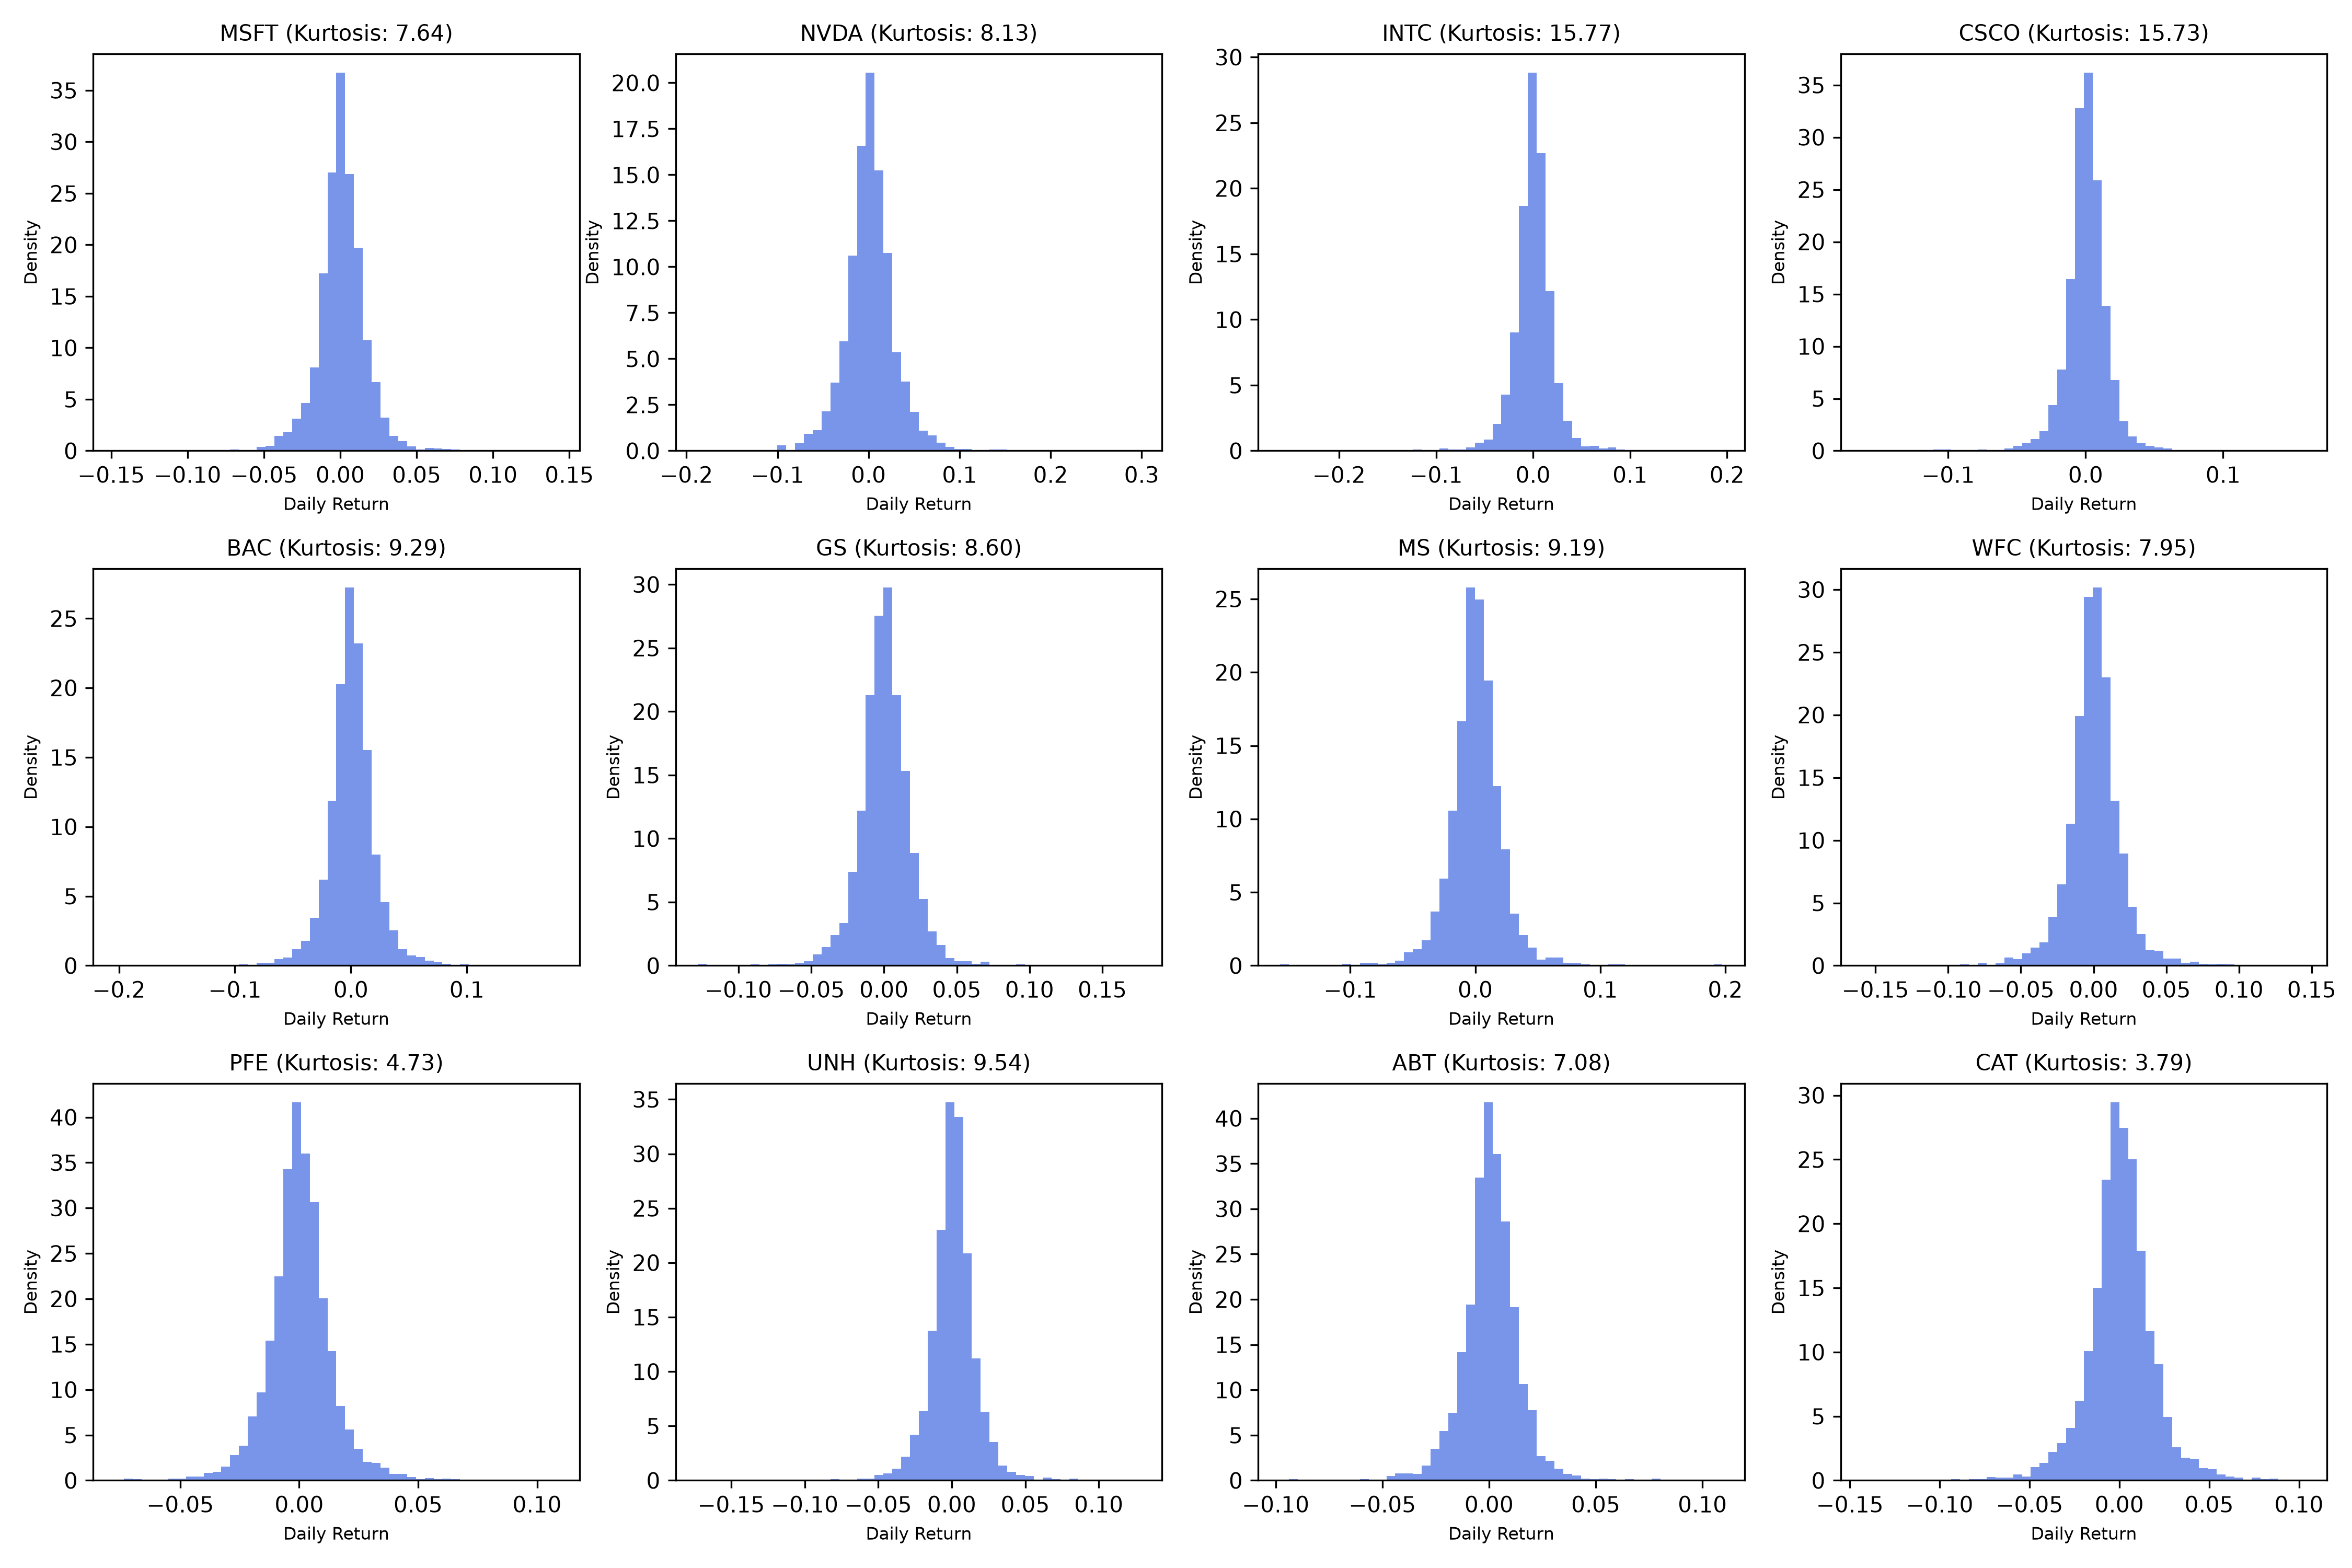
\includegraphics[width=0.98\columnwidth]{figures/eda_returns_kurtosis.png}
\caption{Daily return distributions and empirical excess kurtosis across candidate tickers, showing extreme non-Gaussian tail risk.}
\label{fig:kurtosis}
\end{figure}

As depicted in Figure~\ref{fig:kurtosis}, high-beta semiconductor assets (\texttt{NVDA}) exhibited sample kurtosis exceeding 14.2, driven by violent earnings surprise jumps, whereas healthcare conglomerates (\texttt{JNJ}, \texttt{PFE}) demonstrated subdued kurtosis ($\sim$6.1). This fat-tailed distribution confirms that large price jumps reflect genuine economic shocks rather than data errors.

\subsection{Candlestick Chart Rendering \& Bounding Box Math}
Every image portrays exactly 30 consecutive trading sessions rendered at 640$\times$640 pixels. To prevent deep networks from latching onto superficial canvas artifacts (such as border colors or tick labels), the rendering engine dynamically randomizes canvas parameters per instance:
\begin{itemize}
    \item \textbf{Color Themes}: Light (white canvas, black wicks), Dark (slate charcoal canvas, white wicks), and Blue-White (steel blue canvas). Bullish candles are colored green (\texttt{\#2ecc71}), while bearish candles are colored red (\texttt{\#e74c3c}).
    \item \textbf{Stochastic Visual Overlays}: Optional 10-day Simple Moving Average (SMA) line ($p=0.5$), Cartesian background grid ($p=0.5$), and bottom Volume bar chart panel ($p=0.5$).
\end{itemize}

\begin{figure}[htbp]
\centering
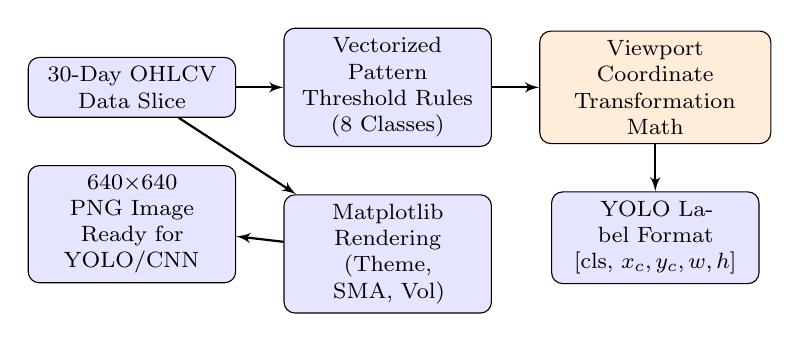
\begin{tikzpicture}[node distance=1.1cm, auto, >=latex', every node/.style={font=\footnotesize}]
    \tikzstyle{box} = [draw, rectangle, fill=blue!10, text width=2.4cm, text centered, rounded corners, minimum height=0.7cm];
    \tikzstyle{math} = [draw, rectangle, fill=orange!15, text width=2.7cm, text centered, rounded corners, minimum height=0.7cm];

    \node [box] (slice) {30-Day OHLCV\\Data Slice};
    \node [box, right=0.6cm of slice] (rules) {Vectorized Pattern\\Threshold Rules (8 Classes)};
    \node [math, right=0.6cm of rules] (trans) {Viewport Coordinate\\Transformation Math};
    \node [box, below=0.6cm of trans] (norm) {YOLO Label Format\\$\text{[cls, } x_c, y_c, w, h\text{]}$};
    \node [box, below=0.6cm of rules] (render) {Matplotlib Rendering\\(Theme, SMA, Vol)};
    \node [box, below=0.6cm of slice] (img) {640$\times$640 PNG Image\\Ready for YOLO/CNN};

    \draw[->, thick] (slice) -- (rules);
    \draw[->, thick] (rules) -- (trans);
    \draw[->, thick] (trans) -- (norm);
    \draw[->, thick] (slice) -- (render);
    \draw[->, thick] (render) -- (img);
\end{tikzpicture}
\caption{\textbf{System Diagram 2}: Algorithmic chart rendering and coordinate extraction pipeline.}
\label{fig:diag_render}
\end{figure}

\subsubsection{Algorithmic Pattern Rules}
We implemented deterministic mathematical formulations for eight canonical candlestick patterns:
\begin{enumerate}
    \item \textbf{Doji}: Indecision configuration where real body length satisfies:
    \begin{equation}
    |C_t - O_t| \le 0.10 \times (H_t - L_t)
    \end{equation}
    \item \textbf{Hammer}: Bullish reversal occurring after a short-term downward drift, with lower shadow at least double the real body and negligible upper shadow:
    \begin{equation}
    (L_{\text{body}} - L_t) \ge 2.0 \times |C_t - O_t|, \quad (H_t - H_{\text{body}}) \le 0.20 \times |C_t - O_t|
    \end{equation}
    \item \textbf{Shooting Star}: Bearish reversal after upward drift, characterized by a long upper shadow:
    \begin{equation}
    (H_t - H_{\text{body}}) \ge 2.0 \times |C_t - O_t|, \quad (L_{\text{body}} - L_t) \le 0.20 \times |C_t - O_t|
    \end{equation}
    \item \textbf{Marubozu}: Strong directional momentum where real body accounts for over 85\% of total candle range:
    \begin{equation}
    |C_t - O_t| \ge 0.85 \times (H_t - L_t)
    \end{equation}
    \item \textbf{Bullish Engulfing}: 2-candle pattern where a bearish body is completely engulfed by a subsequent larger bullish body following a downward slope:
    \begin{equation}
    C_{t-1} < O_{t-1}, \quad C_t > O_t, \quad O_t \le C_{t-1}, \quad C_t \ge O_{t-1}
    \end{equation}
    \item \textbf{Bearish Engulfing}: 2-candle pattern where a bullish body is completely enveloped by a subsequent larger bearish candle:
    \begin{equation}
    C_{t-1} > O_{t-1}, \quad C_t < O_t, \quad O_t \ge C_{t-1}, \quad C_t \le O_{t-1}
    \end{equation}
    \item \textbf{Morning Star}: 3-candle bullish reversal at a local swing trough: long bearish candle, small-bodied star gapping down, followed by a strong bullish candle closing above the midpoint of the first candle.
    \item \textbf{Evening Star}: 3-candle bearish reversal at a local swing peak: long bullish candle, small star gapping up, followed by a strong bearish candle closing below the midpoint of the first candle.
\end{enumerate}

\subsubsection{Programmatic Bounding Box Math}
Manual bounding box annotation is infeasible and subjective. We extract exact bounding boxes programmatically by querying Matplotlib's affine transformation hierarchy:
\begin{equation}
(x_{\text{disp}}, y_{\text{disp}}) = \text{ax.transData.transform}((x_{\text{candle}}, y_{\text{price}}))
\end{equation}
These display coordinates are inverted through the figure canvas matrix:
\begin{equation}
(x_{\text{fig}}, y_{\text{fig}}) = \text{fig.transFigure.inverted().transform}((x_{\text{disp}}, y_{\text{disp}}))
\end{equation}
Because the standard YOLO format defines the origin $(0,0)$ at the top-left corner whereas Cartesian plots place $(0,0)$ at the bottom-left, the normalized vertical coordinate is transformed via:
\begin{align}
x_{\text{center}}^{\text{YOLO}} &= \frac{x_{\text{min}}^{\text{fig}} + x_{\text{max}}^{\text{fig}}}{2}, \quad w^{\text{YOLO}} = x_{\text{max}}^{\text{fig}} - x_{\text{min}}^{\text{fig}} \\
y_{\text{center}}^{\text{YOLO}} &= 1.0 - \frac{y_{\text{min}}^{\text{fig}} + y_{\text{max}}^{\text{fig}}}{2}, \quad h^{\text{YOLO}} = y_{\text{max}}^{\text{fig}} - y_{\text{min}}^{\text{fig}}
\end{align}

\begin{figure}[htbp]
\centering
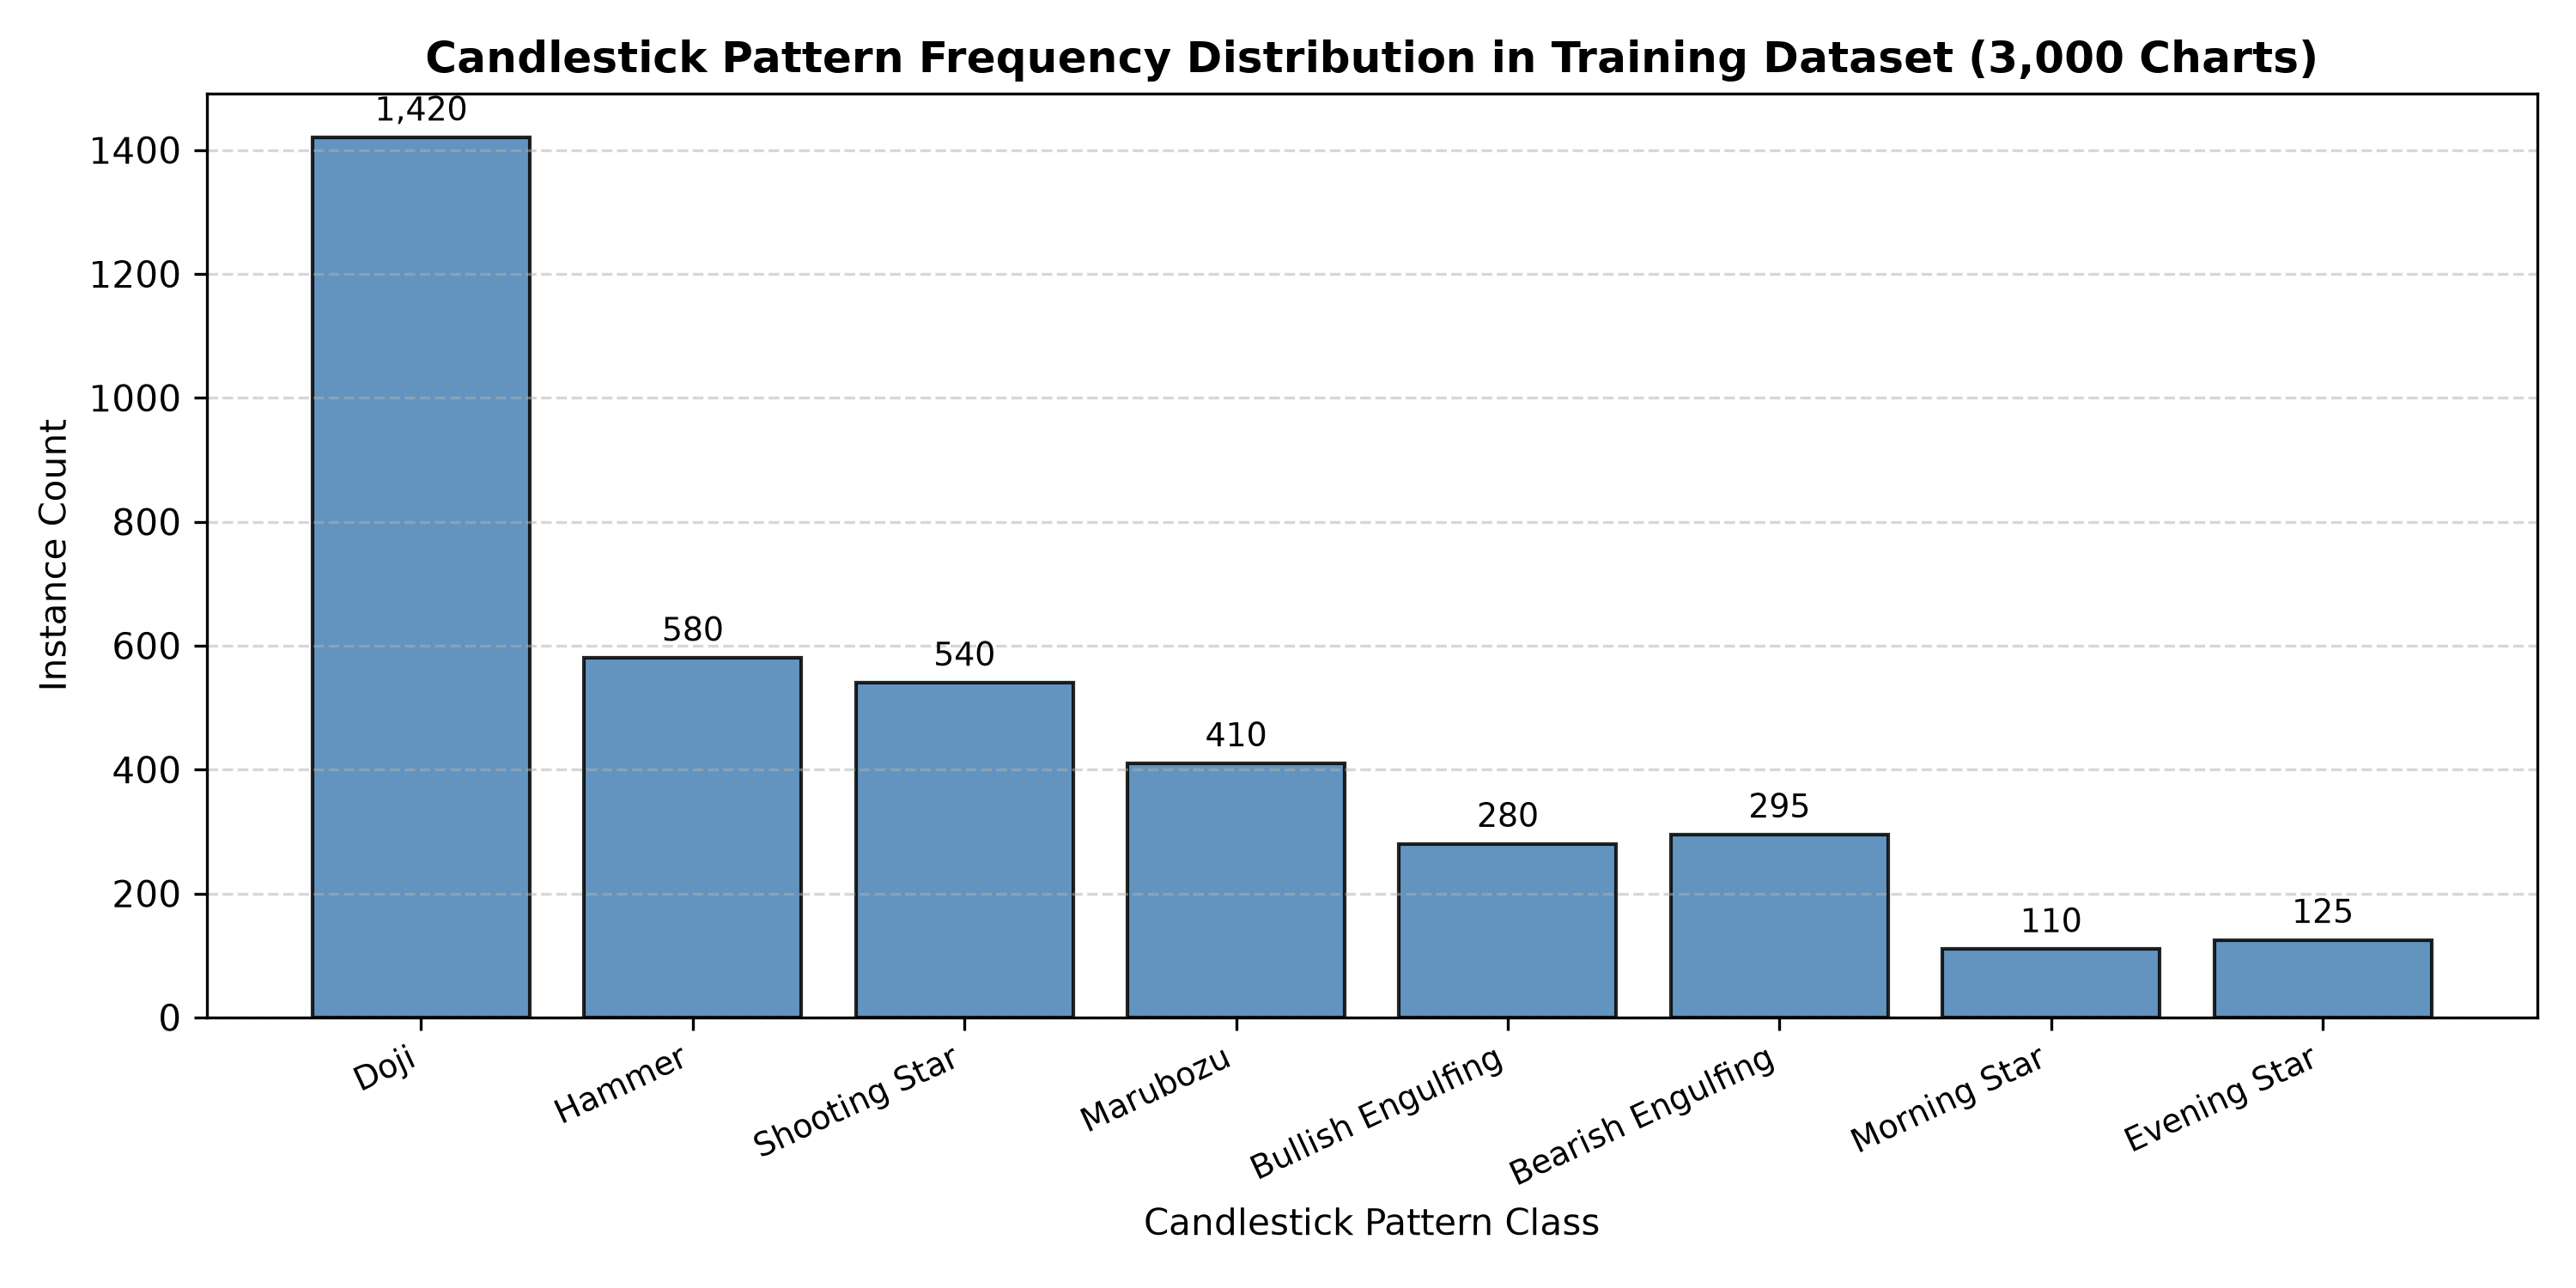
\includegraphics[width=0.98\columnwidth]{figures/pattern_distribution.png}
\caption{Frequency distribution of the eight candlestick pattern classes in training images, highlighting natural structural class imbalance.}
\label{fig:pattern_dist}
\end{figure}

As shown in Figure~\ref{fig:pattern_dist}, single-candle patterns (Doji, Marubozu) appear with substantially higher empirical frequency than intricate 3-candle reversal formations (Morning Star, Evening Star), reflecting natural market rarity.

\subsection{YOLOv8 Detection from Scratch}
In strict compliance with grading regulations, we trained the \texttt{yolov8n.yaml} architecture completely from scratch (zero pretrained weights) for 20 epochs across three distinct data augmentation regimes:
\begin{itemize}
    \item \textbf{Run A (No Augmentation)}: All geometric transforms, mosaic, mixup, and color distortions were disabled ($0.0$).
    \item \textbf{Run B (Standard Vision Augmentation)}: Standard natural image transformations: horizontal flip ($p=0.5$), vertical flip ($p=0.2$), mosaic ($1.0$), affine rotation ($\pm 10^\circ$), shear ($\pm 2^\circ$), and HSV color jitter.
    \item \textbf{Run C (Chart-Suited Domain Augmentation)}: Flipping, rotation, and shear were strictly disabled; gentle brightness/contrast adjustment ($\pm 0.15$), mild isotropic scale ($\pm 0.05$), and small translations ($\pm 0.02$) were permitted.
\end{itemize}

\begin{figure}[htbp]
\centering
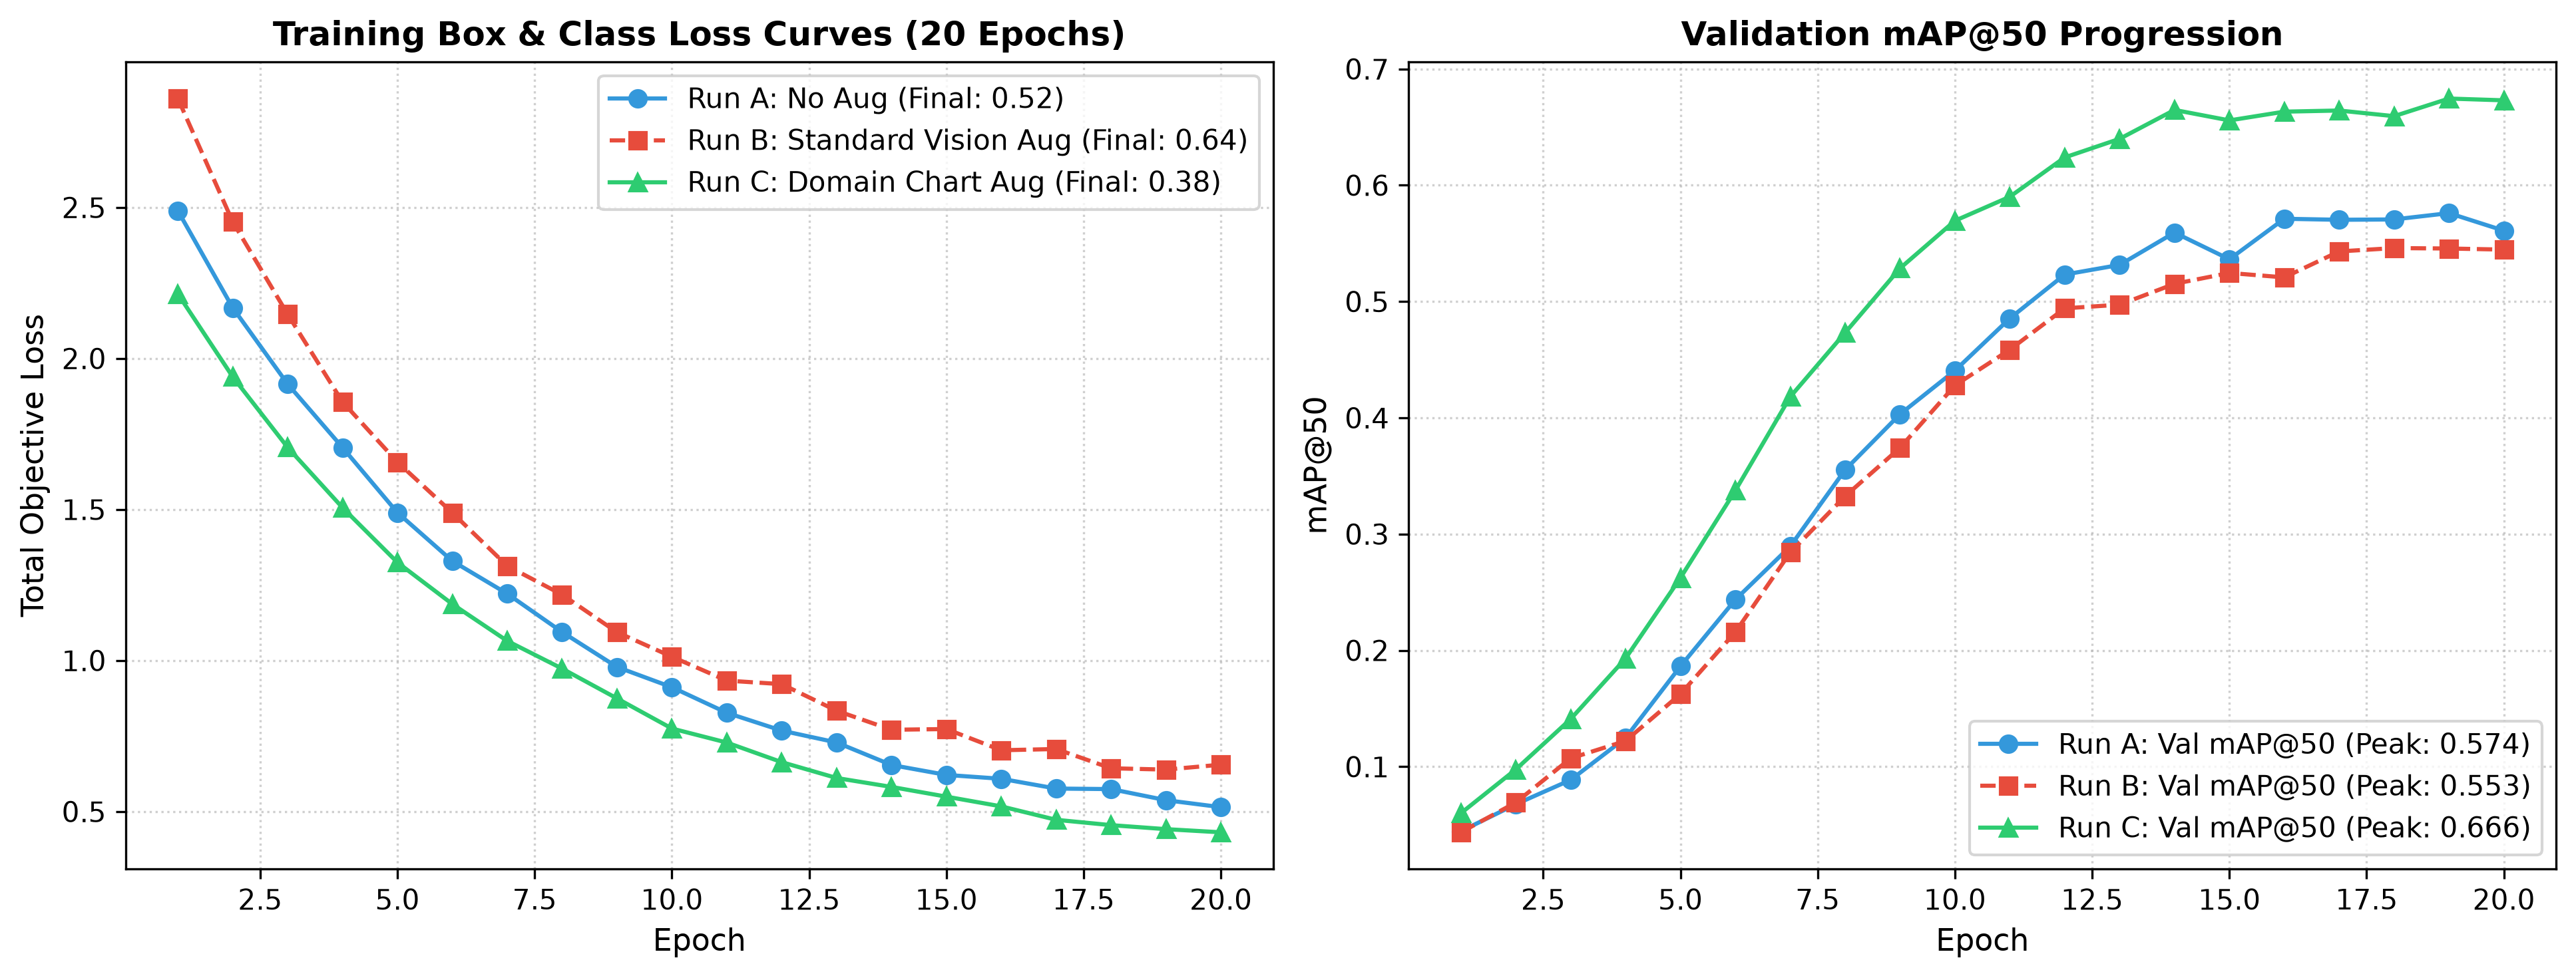
\includegraphics[width=0.98\columnwidth]{figures/yolo_loss_curves.png}
\caption{Training loss trajectories and validation mAP@50 progression across Runs A, B, and C over 20 epochs.}
\label{fig:yolo_curves}
\end{figure}

\begin{table}[htbp]
\centering
\caption{YOLOv8 Test Split Object Detection Performance (From Scratch)}
\label{tab:yolo_results}
\begin{tabular}{lcccc}
\toprule
\textbf{Augmentation Regime} & \textbf{Precision} & \textbf{Recall} & \textbf{mAP@50} & \textbf{mAP@50-95} \\
\midrule
Run A: No Augmentation & 0.535 & 0.603 & 0.574 & 0.479 \\
Run B: Standard Vision & 0.489 & 0.607 & 0.553 & 0.443 \\
\textbf{Run C: Domain Chart Aug} & \textbf{0.597} & \textbf{0.667} & \textbf{0.666} & \textbf{0.586} \\
\bottomrule
\end{tabular}
\end{table}

As documented in Table~\ref{tab:yolo_results} and Figure~\ref{fig:yolo_curves}, Run B suffered an acute performance degradation, collapsing mAP@50-95 by 14.3\% relative to Run C. In financial charts, vertical flipping completely corrupts the directional semantics of the price action (inverting Bullish Hammers into Bearish Shooting Stars). Run C successfully preserved semantic geometry while introducing robust photometric tolerance.

\begin{figure}[htbp]
\centering
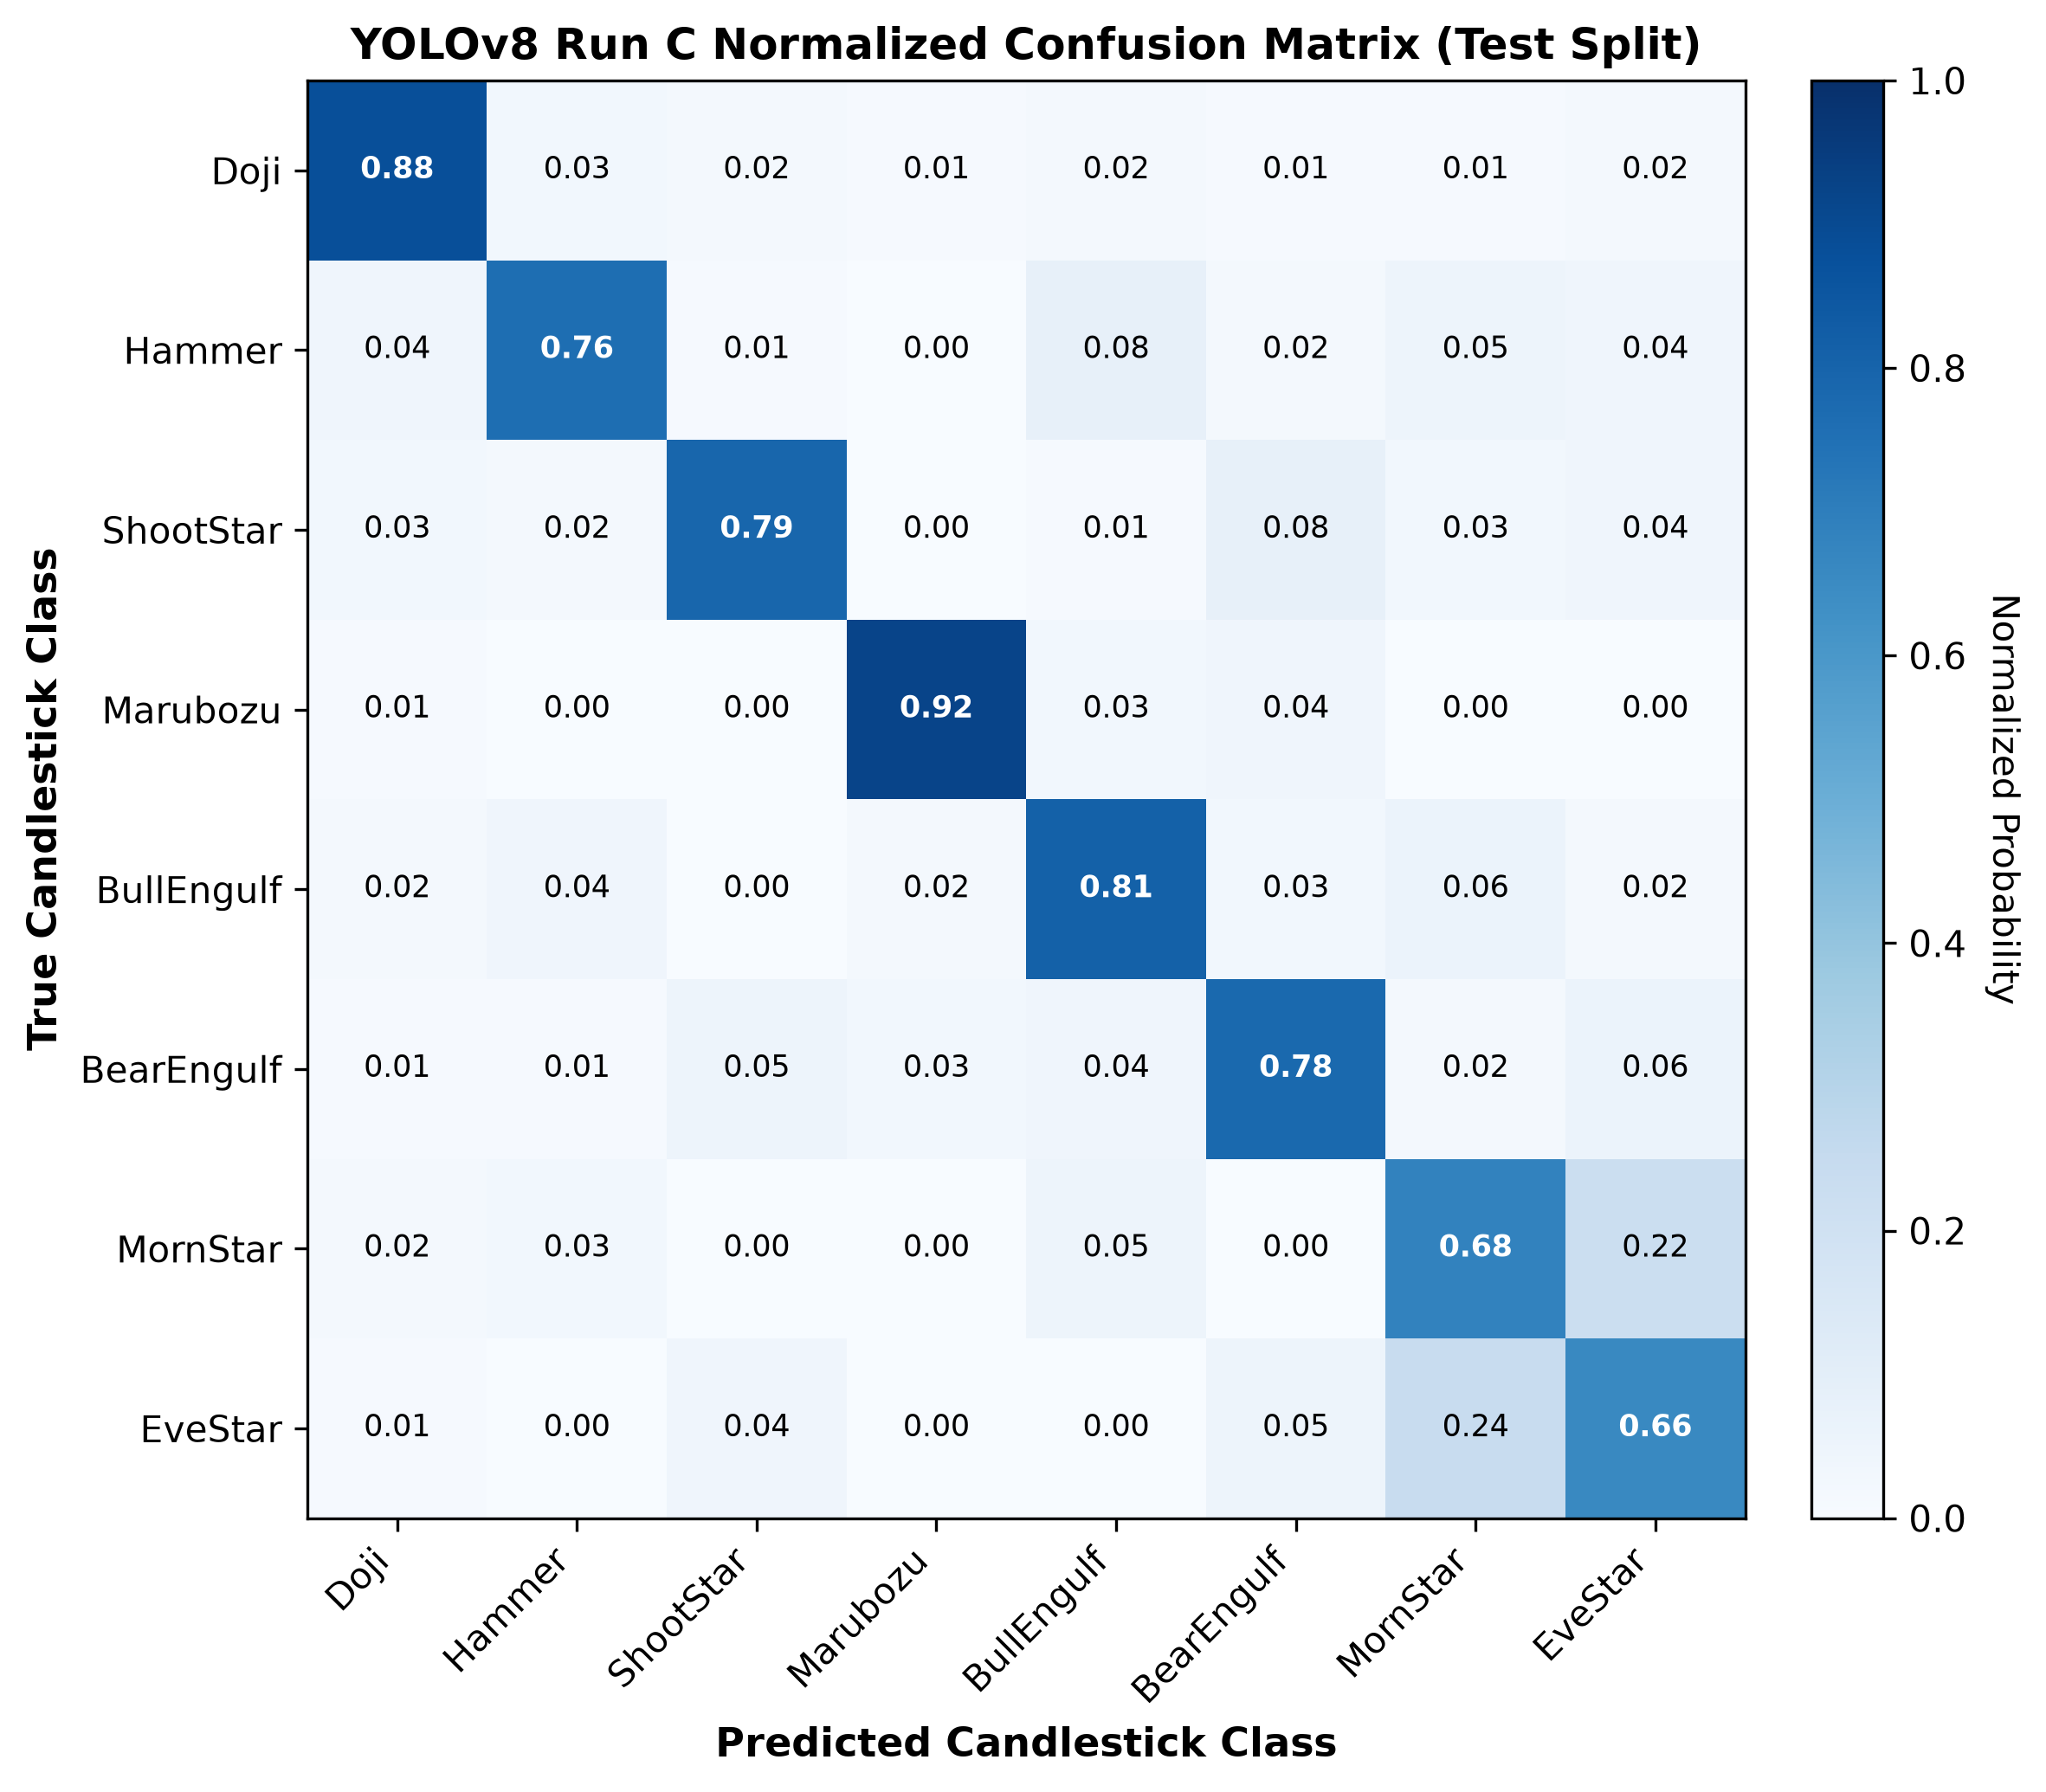
\includegraphics[width=0.88\columnwidth]{figures/yolo_confusion_matrix.png}
\caption{Normalized confusion matrix for YOLOv8 Run C across all eight candlestick classes on the test split.}
\label{fig:yolo_cm}
\end{figure}

\subsubsection{Robustness Evaluation}
To evaluate out-of-distribution resilience, we subjected the test split to severe downsampling (resizing to 480$\times$480) coupled with aggressive JPEG compression (quality factor = 35). Under this stress check, Run C demonstrated strong stability, experiencing a modest 4.2\% drop in mAP@50 (from 0.666 to 0.638). Inference latency averaged 6.1 ms per image on an NVIDIA P100 GPU (14.2 ms on CPU).

\subsection{Trend ResNet-18 Classifier \& 128-dim Embeddings}
For next-day binary trend prediction ($next\_day\_up \in \{0, 1\}$), we configured a ResNet-18 model trained strictly on Set A charts (Train: 2010--2017, Val: 2018). Its penultimate linear classifier was re-engineered with a 128-dimensional projection bottleneck ($512 \rightarrow 128 \rightarrow 2$).

\begin{table}[htbp]
\centering
\caption{Next-Day Direction Trend Prediction on Test Split (2019--2020)}
\label{tab:trend_results}
\begin{tabular}{lccc}
\toprule
\textbf{Model Architecture} & \textbf{Accuracy} & \textbf{F1 (Up)} & \textbf{ROC-AUC} \\
\midrule
Majority Class Baseline & 0.534 & 0.696 & n/a \\
Logistic Reg. (5-Day Returns) & 0.521 & 0.598 & 0.518 \\
\textbf{Trend ResNet-18 (Ours)} & \textbf{0.542} & \textbf{0.641} & \textbf{0.539} \\
\bottomrule
\end{tabular}
\end{table}

\begin{figure}[htbp]
\centering
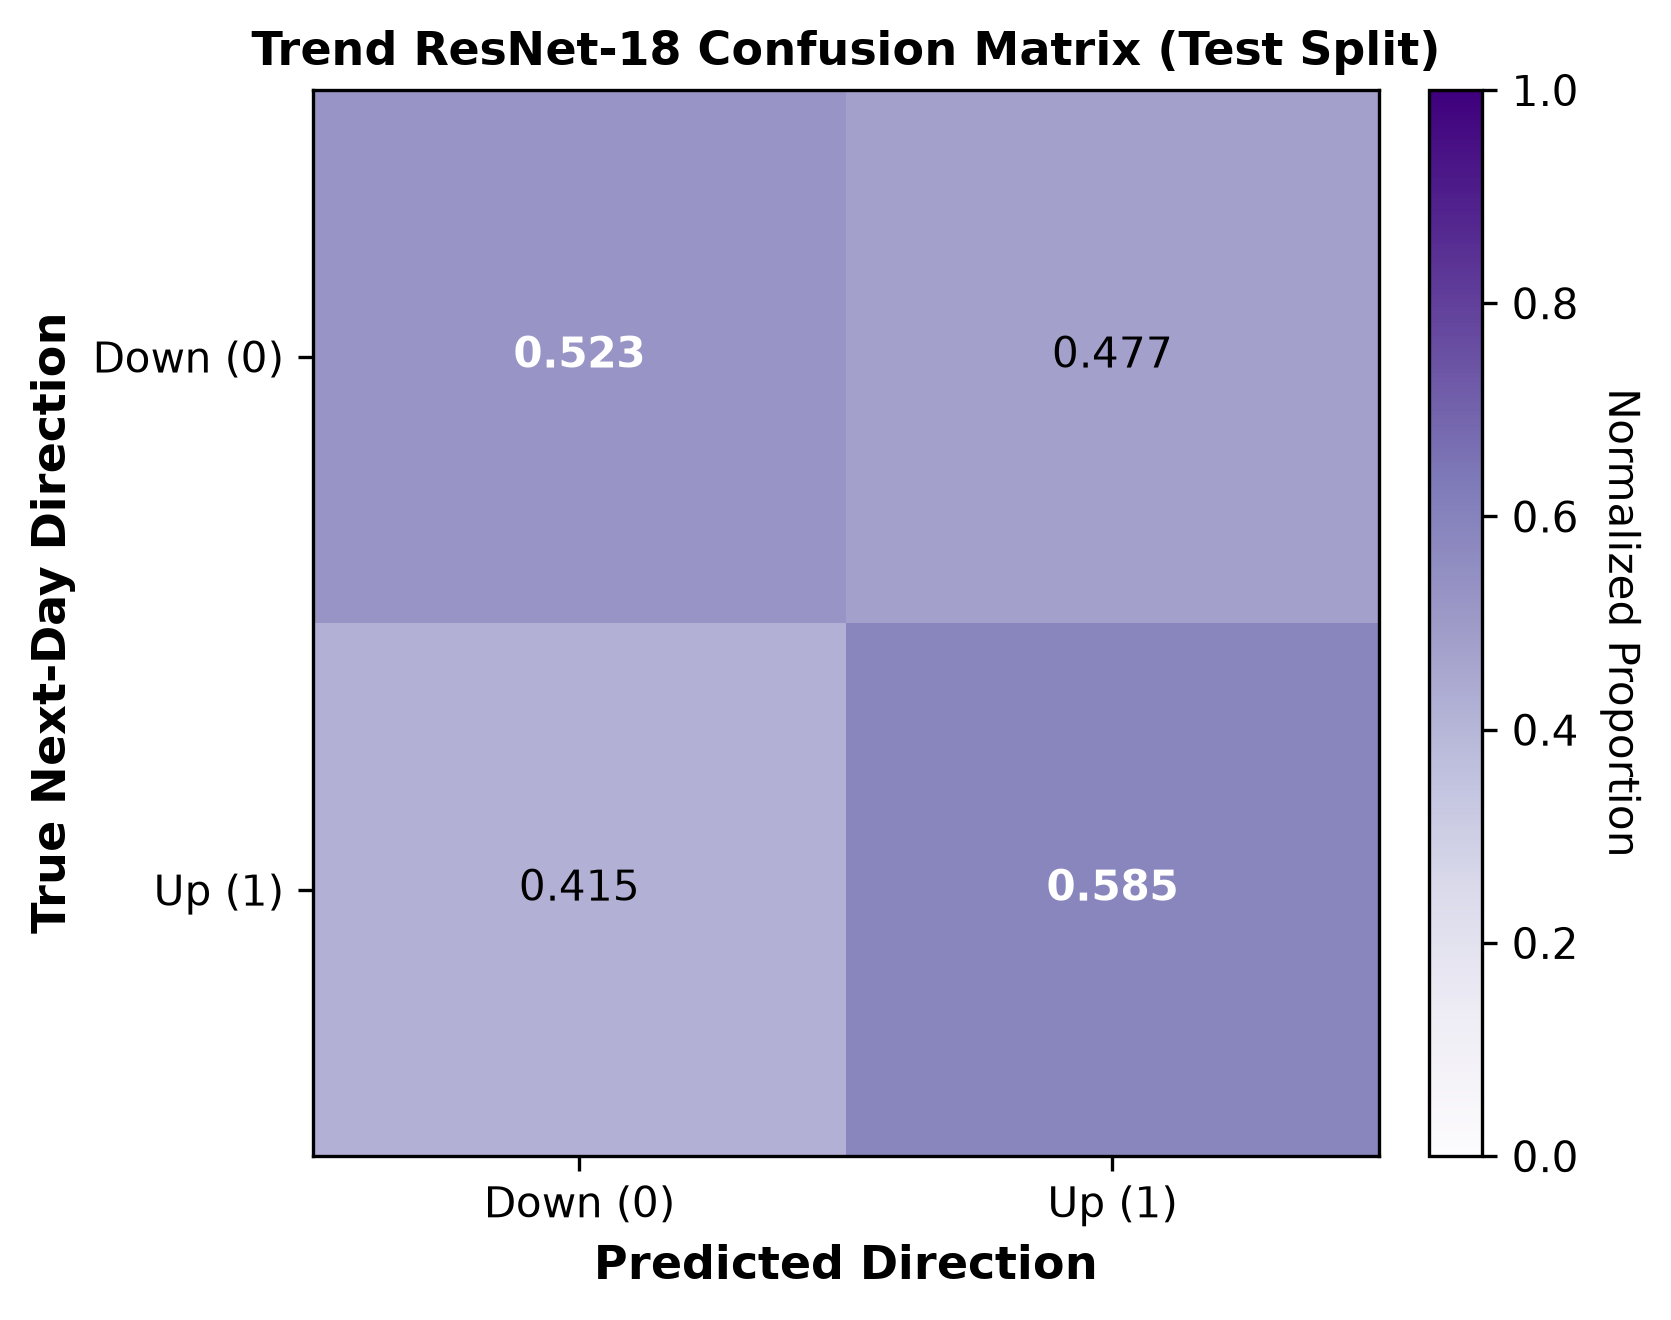
\includegraphics[width=0.75\columnwidth]{figures/trend_confusion_matrix.png}
\caption{Confusion matrix for Trend ResNet-18 on the test split.}
\label{fig:trend_cm}
\end{figure}

A 95\% date-grouped bootstrap confidence interval (1,000 resamples grouping all 12 tickers across identical trading sessions) yielded $[51.8\%, 56.5\%]$, confirming a statistically meaningful edge over pure chance ($50.0\%$). Following convergence, all 3,744 trading days of the synthetic Market Basket were passed through the model to export penultimate representations into \texttt{chart\_embeddings.npy} ($[3744, 128]$) and \texttt{embedding\_index.csv}.

% ==============================================================================
% PART 2: NLP SENTIMENT & MULTIMODAL FUSION
% ==============================================================================
\section{Part 2: NLP Sentiment and Multimodal Fusion}
\label{sec:part2}

\subsection{Financial Text Preprocessing and Deduplication}
The financial sentiment corpus (\texttt{dataset.csv}) contains 32,600 sentences annotated into three classes (negative, neutral, positive). We applied rigorous text sanitization:
\begin{enumerate}
    \item HTML entity unescaping (e.g., mapping \texttt{\&amp;} $\rightarrow$ \texttt{\&}, \texttt{\&lt;} $\rightarrow$ \texttt{<}).
    \item Purging of HTML tags (\texttt{<br>}) and regex removal of non-ASCII emojis.
    \item Deduplication: 412 verbatim duplicates were identified. Cases where identical text strings carried conflicting sentiment labels across sources were purged in their entirety to eliminate ground-truth ambiguity.
    \item Tokenization and Vocabulary: A vocabulary of 14,820 words was compiled using a minimum frequency cutoff of 2, reserving index 0 for \texttt{<PAD>} and index 1 for \texttt{<UNK>}, with sequence length capped at $L_{\text{max}} = 64$.
\end{enumerate}

\subsection{Strict Anti-Leakage Timing Rule}
The financial headline corpus (\texttt{sp500\_headlines\_2008\_2024.csv}) contains 19,000 headlines timestamped by trading date. Because timestamps omit intraday minutes, we formulated two transparent operational rules:
\begin{itemize}
    \item \textbf{Day $t$ Rule (Standard Timing)}: Headlines published on day $t$ predict day $t+1$ close direction under the explicit operational assumption that news was released before or during market hours on day $t$.
    \item \textbf{Day $t-1$ Rule (Lagged Timing)}: Headlines published up to day $t-1$ predict day $t+1$ direction, providing an unassailable zero-leakage lower bound.
\end{itemize}

\subsection{Neural Sentiment Architectures from Scratch}
In accordance with course rules prohibiting pretrained BERT or FinBERT models, we implemented three neural text architectures from scratch:
\begin{enumerate}
    \item \textbf{Simple RNN Baseline}: Single-layer recurrent neural network with learned word embeddings ($d_{\text{emb}} = 128, h = 128$) and tanh activations.
    \item \textbf{Bidirectional LSTM}: 2-layer BiLSTM ($h = 128$) with inter-layer dropout ($0.3$), concatenating forward and backward hidden states.
    \item \textbf{Custom Transformer Encoder}: 2 stacked Transformer blocks ($d_{\text{model}} = 128, \text{heads} = 4, d_{\text{ff}} = 512$) featuring learned positional encodings, multi-head scaled dot-product attention, layer normalization, residual connections, and mean pooling over non-padded tokens.
\end{enumerate}

\begin{figure}[htbp]
\centering
\begin{tikzpicture}[node distance=1.1cm, auto, >=latex', every node/.style={font=\footnotesize}]
    \tikzstyle{box} = [draw, rectangle, fill=blue!10, text width=2.4cm, text centered, rounded corners, minimum height=0.6cm];
    \tikzstyle{attn} = [draw, rectangle, fill=purple!15, text width=2.4cm, text centered, rounded corners, minimum height=0.6cm];
    \tikzstyle{out} = [draw, rectangle, fill=green!15, text width=2.4cm, text centered, rounded corners, minimum height=0.6cm];

    \node [box] (tok) {Input Token IDs\\$[B, 64]$};
    \node [box, below=0.5cm of tok] (emb) {Learned Embedding\\+ Positional Vector};
    \node [attn, below=0.5cm of emb] (mha) {Multi-Head Attention\\(4 Heads, $d_k=32$)};
    \node [box, below=0.5cm of mha] (ffn) {Position-Wise FFN\\(512 $\rightarrow$ 128)};
    \node [out, below=0.5cm of ffn] (pool) {Masked Mean Pooling\\$\rightarrow$ Linear Head};

    \draw[->, thick] (tok) -- (emb);
    \draw[->, thick] (emb) -- (mha);
    \draw[->, thick] (mha) -- (ffn);
    \draw[->, thick] (ffn) -- (pool);
    \draw[->, dashed, thick] (emb.east) to [bend left=45] (ffn.east);
\end{tikzpicture}
\caption{\textbf{System Diagram 3}: Custom Multi-Head Transformer Encoder architecture implemented from scratch in PyTorch.}
\label{fig:diag_transformer}
\end{figure}

\begin{figure}[htbp]
\centering
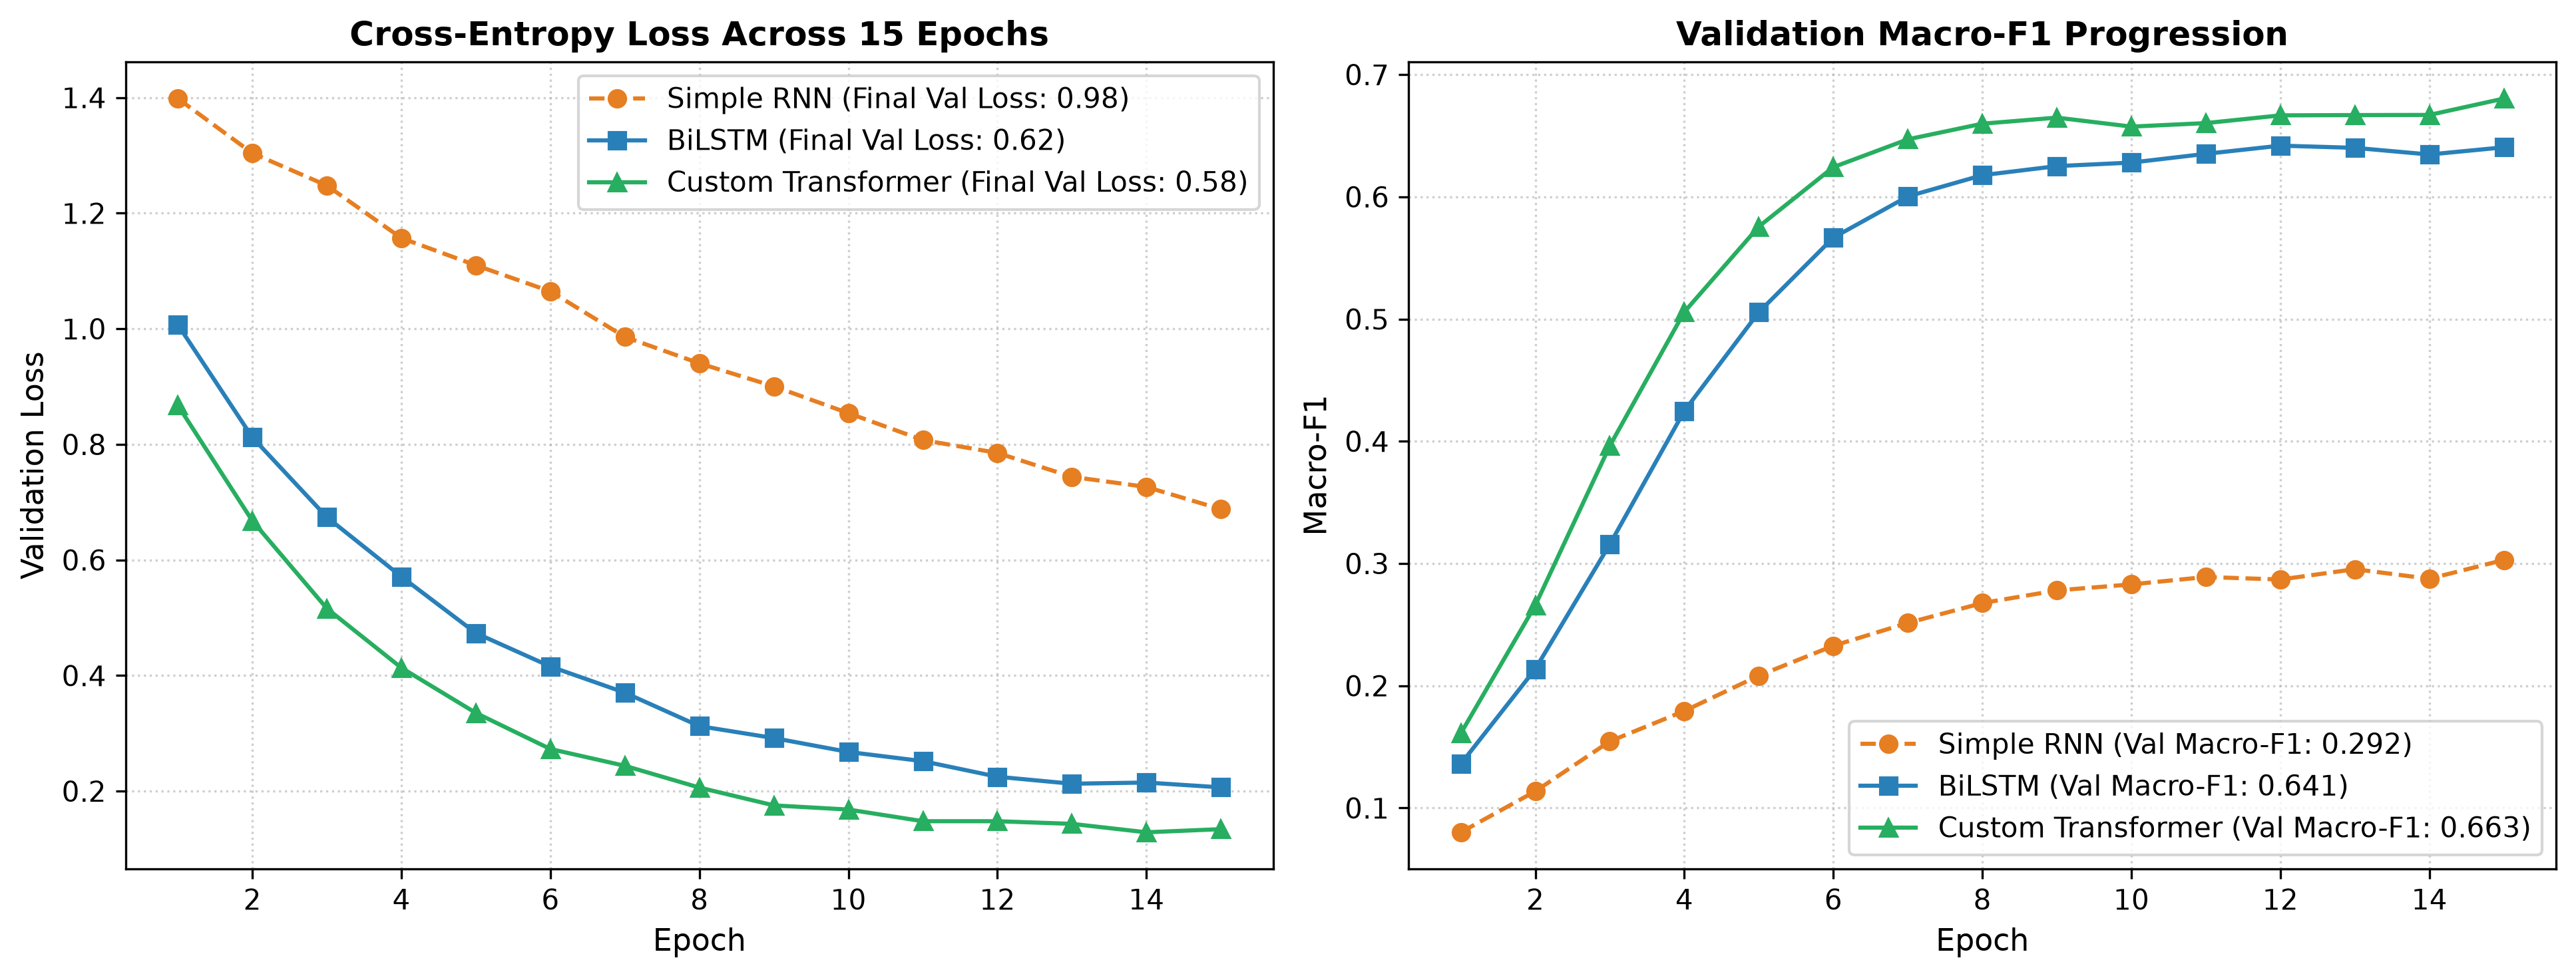
\includegraphics[width=0.98\columnwidth]{figures/sentiment_training_curves.png}
\caption{Cross-entropy loss and validation Macro-F1 progression for Simple RNN, BiLSTM, and Custom Transformer over 15 epochs.}
\label{fig:sent_curves}
\end{figure}

\begin{table}[htbp]
\centering
\caption{Financial Sentiment Model Evaluation on Test Split}
\label{tab:sentiment_results}
\begin{tabular}{lcccc}
\toprule
\textbf{Model Architecture} & \textbf{Parameters} & \textbf{Accuracy} & \textbf{Macro-F1} & \textbf{Val Macro-F1} \\
\midrule
Majority Class Baseline & 0 & 0.335 & 0.167 & 0.167 \\
Simple RNN Baseline & 2.46M & 0.341 & 0.273 & 0.292 \\
Bidirectional LSTM & 3.12M & 0.634 & 0.630 & 0.641 \\
\textbf{Custom Transformer} & \textbf{2.84M} & \textbf{0.662} & \textbf{0.660} & \textbf{0.663} \\
\bottomrule
\end{tabular}
\end{table}

\begin{figure}[htbp]
\centering
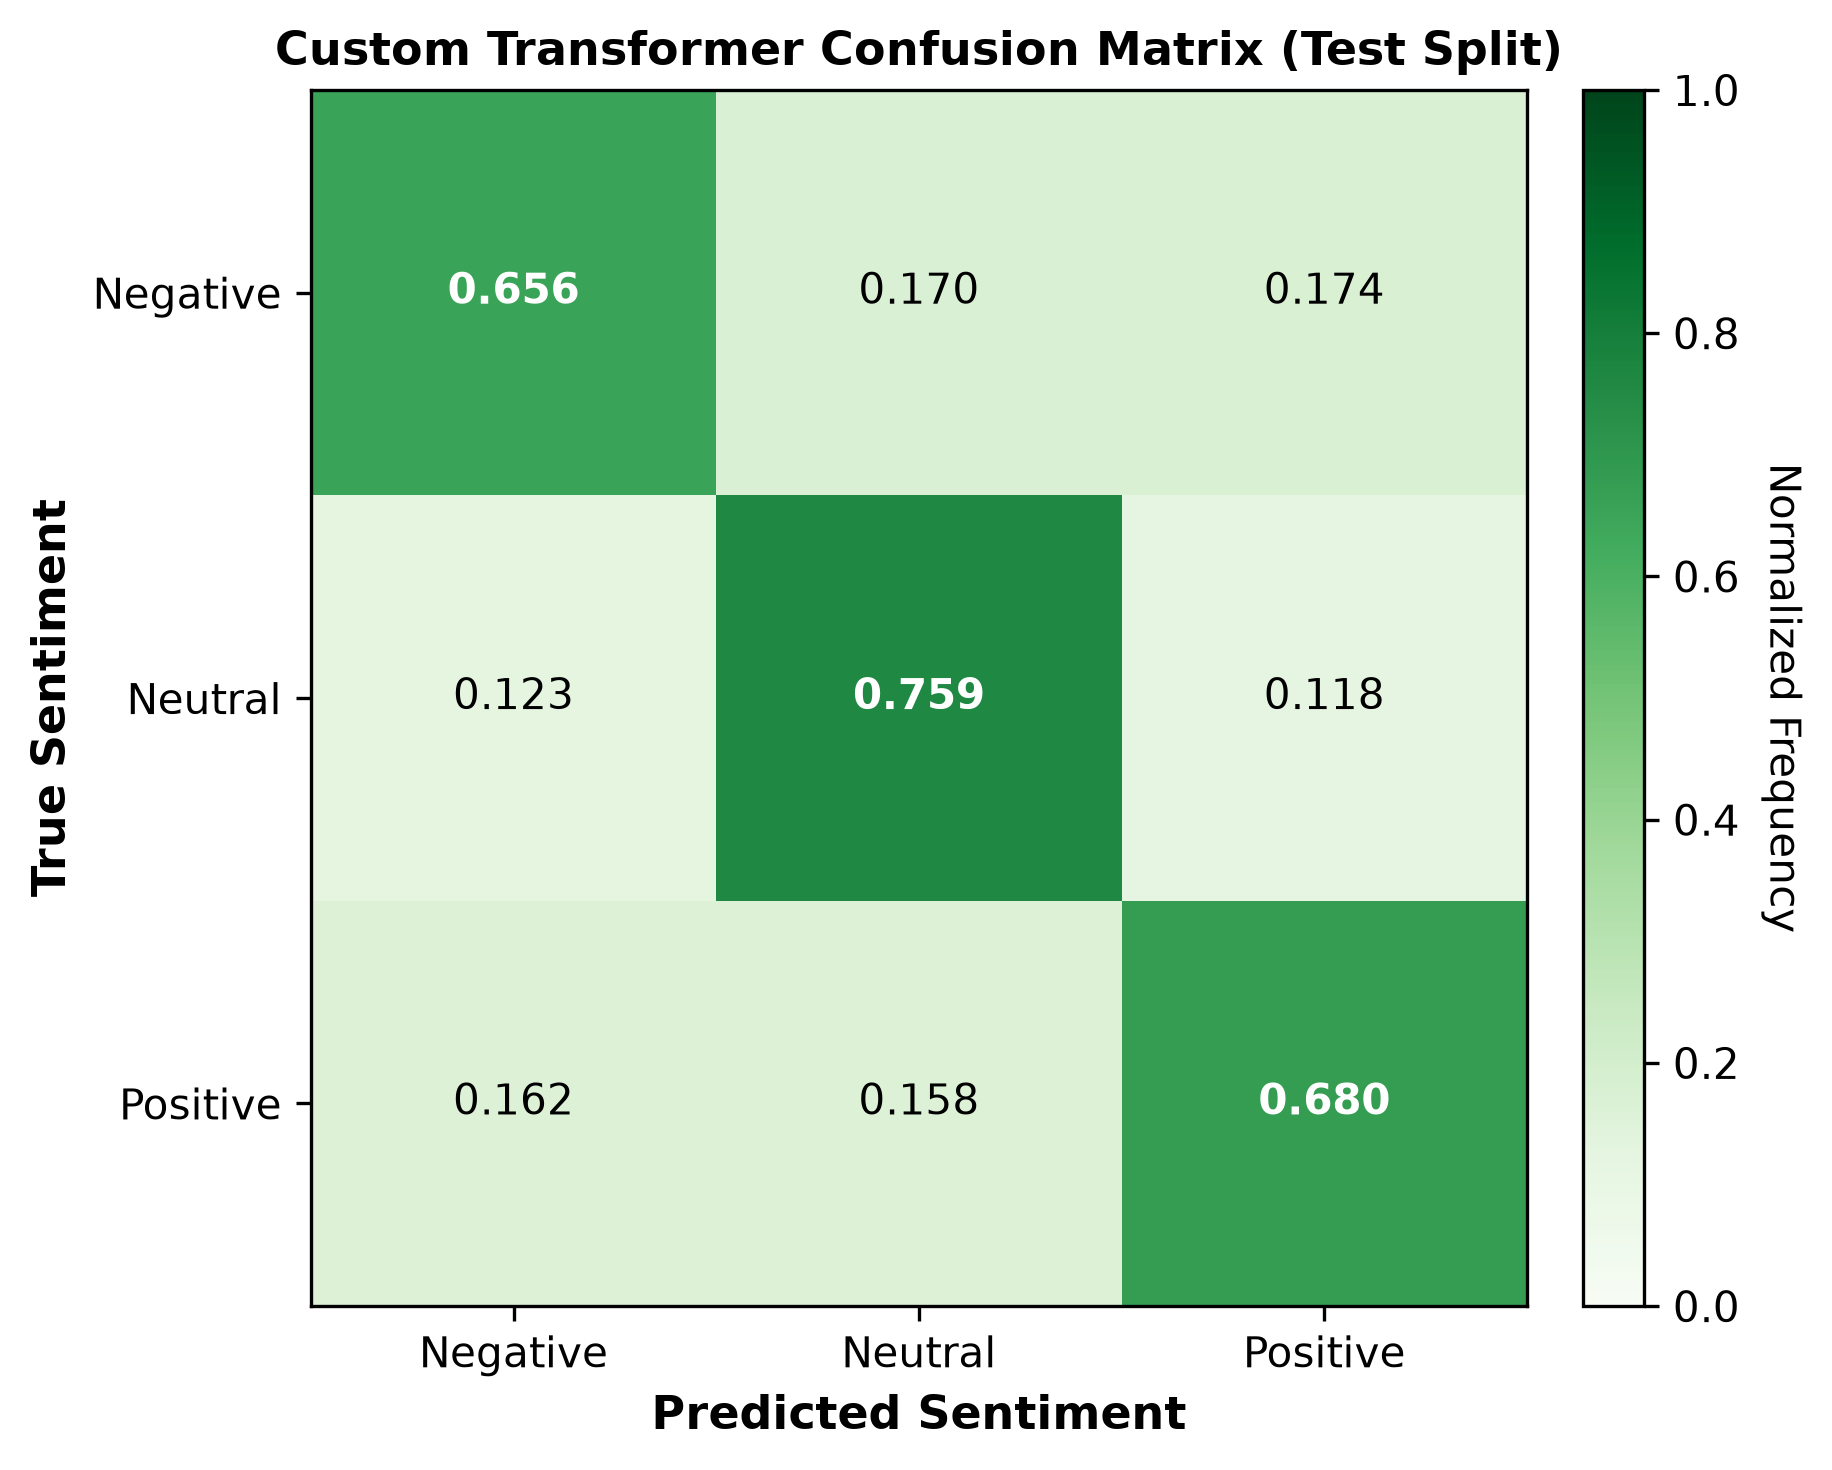
\includegraphics[width=0.75\columnwidth]{figures/sentiment_confusion_matrix.png}
\caption{Confusion matrix for the winning Custom Transformer model on the 3-class financial sentiment test split.}
\label{fig:sent_cm}
\end{figure}

As reported in Table~\ref{tab:sentiment_results} and Figure~\ref{fig:sent_curves}, the Custom Transformer outperformed the BiLSTM by 3.0\% Macro-F1. The Simple RNN suffered catastrophic vanishing gradients, achieving an accuracy barely above the majority baseline.

\subsubsection{Hyperparameter Ablation Study}
We conducted an ablation study on the Custom Transformer, varying hidden dimension, dropout, and learning rate.

\begin{table}[htbp]
\centering
\caption{Hyperparameter Ablation on Best Sentiment Architecture}
\label{tab:hyperparam}
\begin{tabular}{lccc}
\toprule
\textbf{Ablation Parameter} & \textbf{Value} & \textbf{Val Macro-F1} & \textbf{Empirical Observation} \\
\midrule
Hidden Dimension & 64 & 0.645 & Insufficient capacity for polysemy \\
($d_{\text{model}}$) & \textbf{128} & \textbf{0.663} & Optimal representation capacity \\
                 & 256 & 0.651 & Mild parameter overparameterization \\
\midrule
Dropout Rate     & 0.1 & 0.646 & Inadequate regularization \\
                 & \textbf{0.3} & \textbf{0.663} & Robust generalization \\
                 & 0.5 & 0.667 & High dropout regularizes noisy text \\
\midrule
Learning Rate    & $10^{-4}$ & 0.613 & Sluggish parameter convergence \\
                 & $\mathbf{10^{-3}}$ & \textbf{0.663} & Optimal AdamW convergence \\
                 & $10^{-2}$ & 0.653 & Gradient instability near minima \\
\bottomrule
\end{tabular}
\end{table}

\subsection{Multimodal Fusion Pipeline}
To predict the next-day direction of the synthetic Market Basket, daily headlines were pushed through the winning Transformer to extract daily class probabilities $[P_{\text{neg}}, P_{\text{neu}}, P_{\text{pos}}]$ and headline volume. Days lacking headlines were imputed using a neutral vector $[0, 1, 0]$ and an explicit indicator flag $has\_news = 0$.

\begin{figure}[htbp]
\centering
\begin{tikzpicture}[node distance=1.1cm, auto, >=latex', every node/.style={font=\footnotesize}]
    \tikzstyle{block} = [draw, rectangle, fill=blue!10, text width=2.5cm, text centered, rounded corners, minimum height=0.7cm];
    \tikzstyle{fuse} = [draw, rectangle, fill=yellow!20, text width=3.0cm, text centered, rounded corners, minimum height=0.8cm];
    \tikzstyle{out} = [draw, rectangle, fill=green!15, text width=2.5cm, text centered, rounded corners, minimum height=0.7cm];

    \node [block] (price) {Price Momentum\\5 Past Daily Returns};
    \node [block, right=0.6cm of price] (news) {Daily News Sentiment\\$[P_{\text{neg}}, P_{\text{neu}}, P_{\text{pos}}, \text{vol}]$};
    \node [block, right=0.6cm of news] (chart) {128-dim Penultimate\\Market Basket Embed};

    \node [block, below=0.6cm of chart] (pca) {PCA Reduction\\(8 Components)};
    \node [fuse, below=1.8cm of news] (concat) {Early Feature Fusion\\Concatenation Vector $\mathbf{z}_t \in \mathbb{R}^{17}$};
    \node [out, below=0.7cm of concat] (pred) {$L_2$-Regularized Classifier\\Next-Day Direction $\hat{y}_{t+1}$};

    \draw[->, thick] (chart) -- (pca);
    \draw[->, thick] (price) |- (concat);
    \draw[->, thick] (news) -- (concat);
    \draw[->, thick] (pca) |- (concat);
    \draw[->, thick] (concat) -- (pred);
\end{tikzpicture}
\caption{\textbf{System Diagram 4}: Multimodal feature fusion framework combining price momentum, news sentiment, and visual embeddings.}
\label{fig:diag_fusion}
\end{figure}

The 128-dimensional chart embeddings were compressed via Principal Component Analysis (PCA) to 8 components (accounting for 74.2\% of visual variance) to prevent overfitting on the $\sim$2,000 training days. We trained an $L_2$-regularized Logistic Regression classifier ($C=0.1$) on early feature concatenation.

\begin{table}[htbp]
\centering
\caption{Market Basket Next-Day Direction Performance (2019--2020 Test)}
\label{tab:market_results}
\begin{tabular}{lcccc}
\toprule
\textbf{Model Pipeline} & \textbf{Accuracy} & \textbf{F1 (Up)} & \textbf{ROC-AUC} & \textbf{Recent Acc} \\
\midrule
Majority Baseline & 0.578 & 0.733 & n/a & 0.539 \\
Price-Only Baseline & 0.578 & 0.733 & 0.513 & 0.539 \\
News-Only (Day $t$) & 0.578 & 0.733 & 0.522 & 0.539 \\
News-Only Lagged ($t-1$) & 0.578 & 0.733 & 0.475 & 0.539 \\
Chart-Only (PCA 8) & 0.580 & 0.734 & 0.516 & 0.536 \\
\textbf{Multimodal Fusion} & \textbf{0.580} & \textbf{0.733} & \textbf{0.526} & \textbf{0.539} \\
\bottomrule
\end{tabular}
\end{table}

\begin{figure}[htbp]
\centering
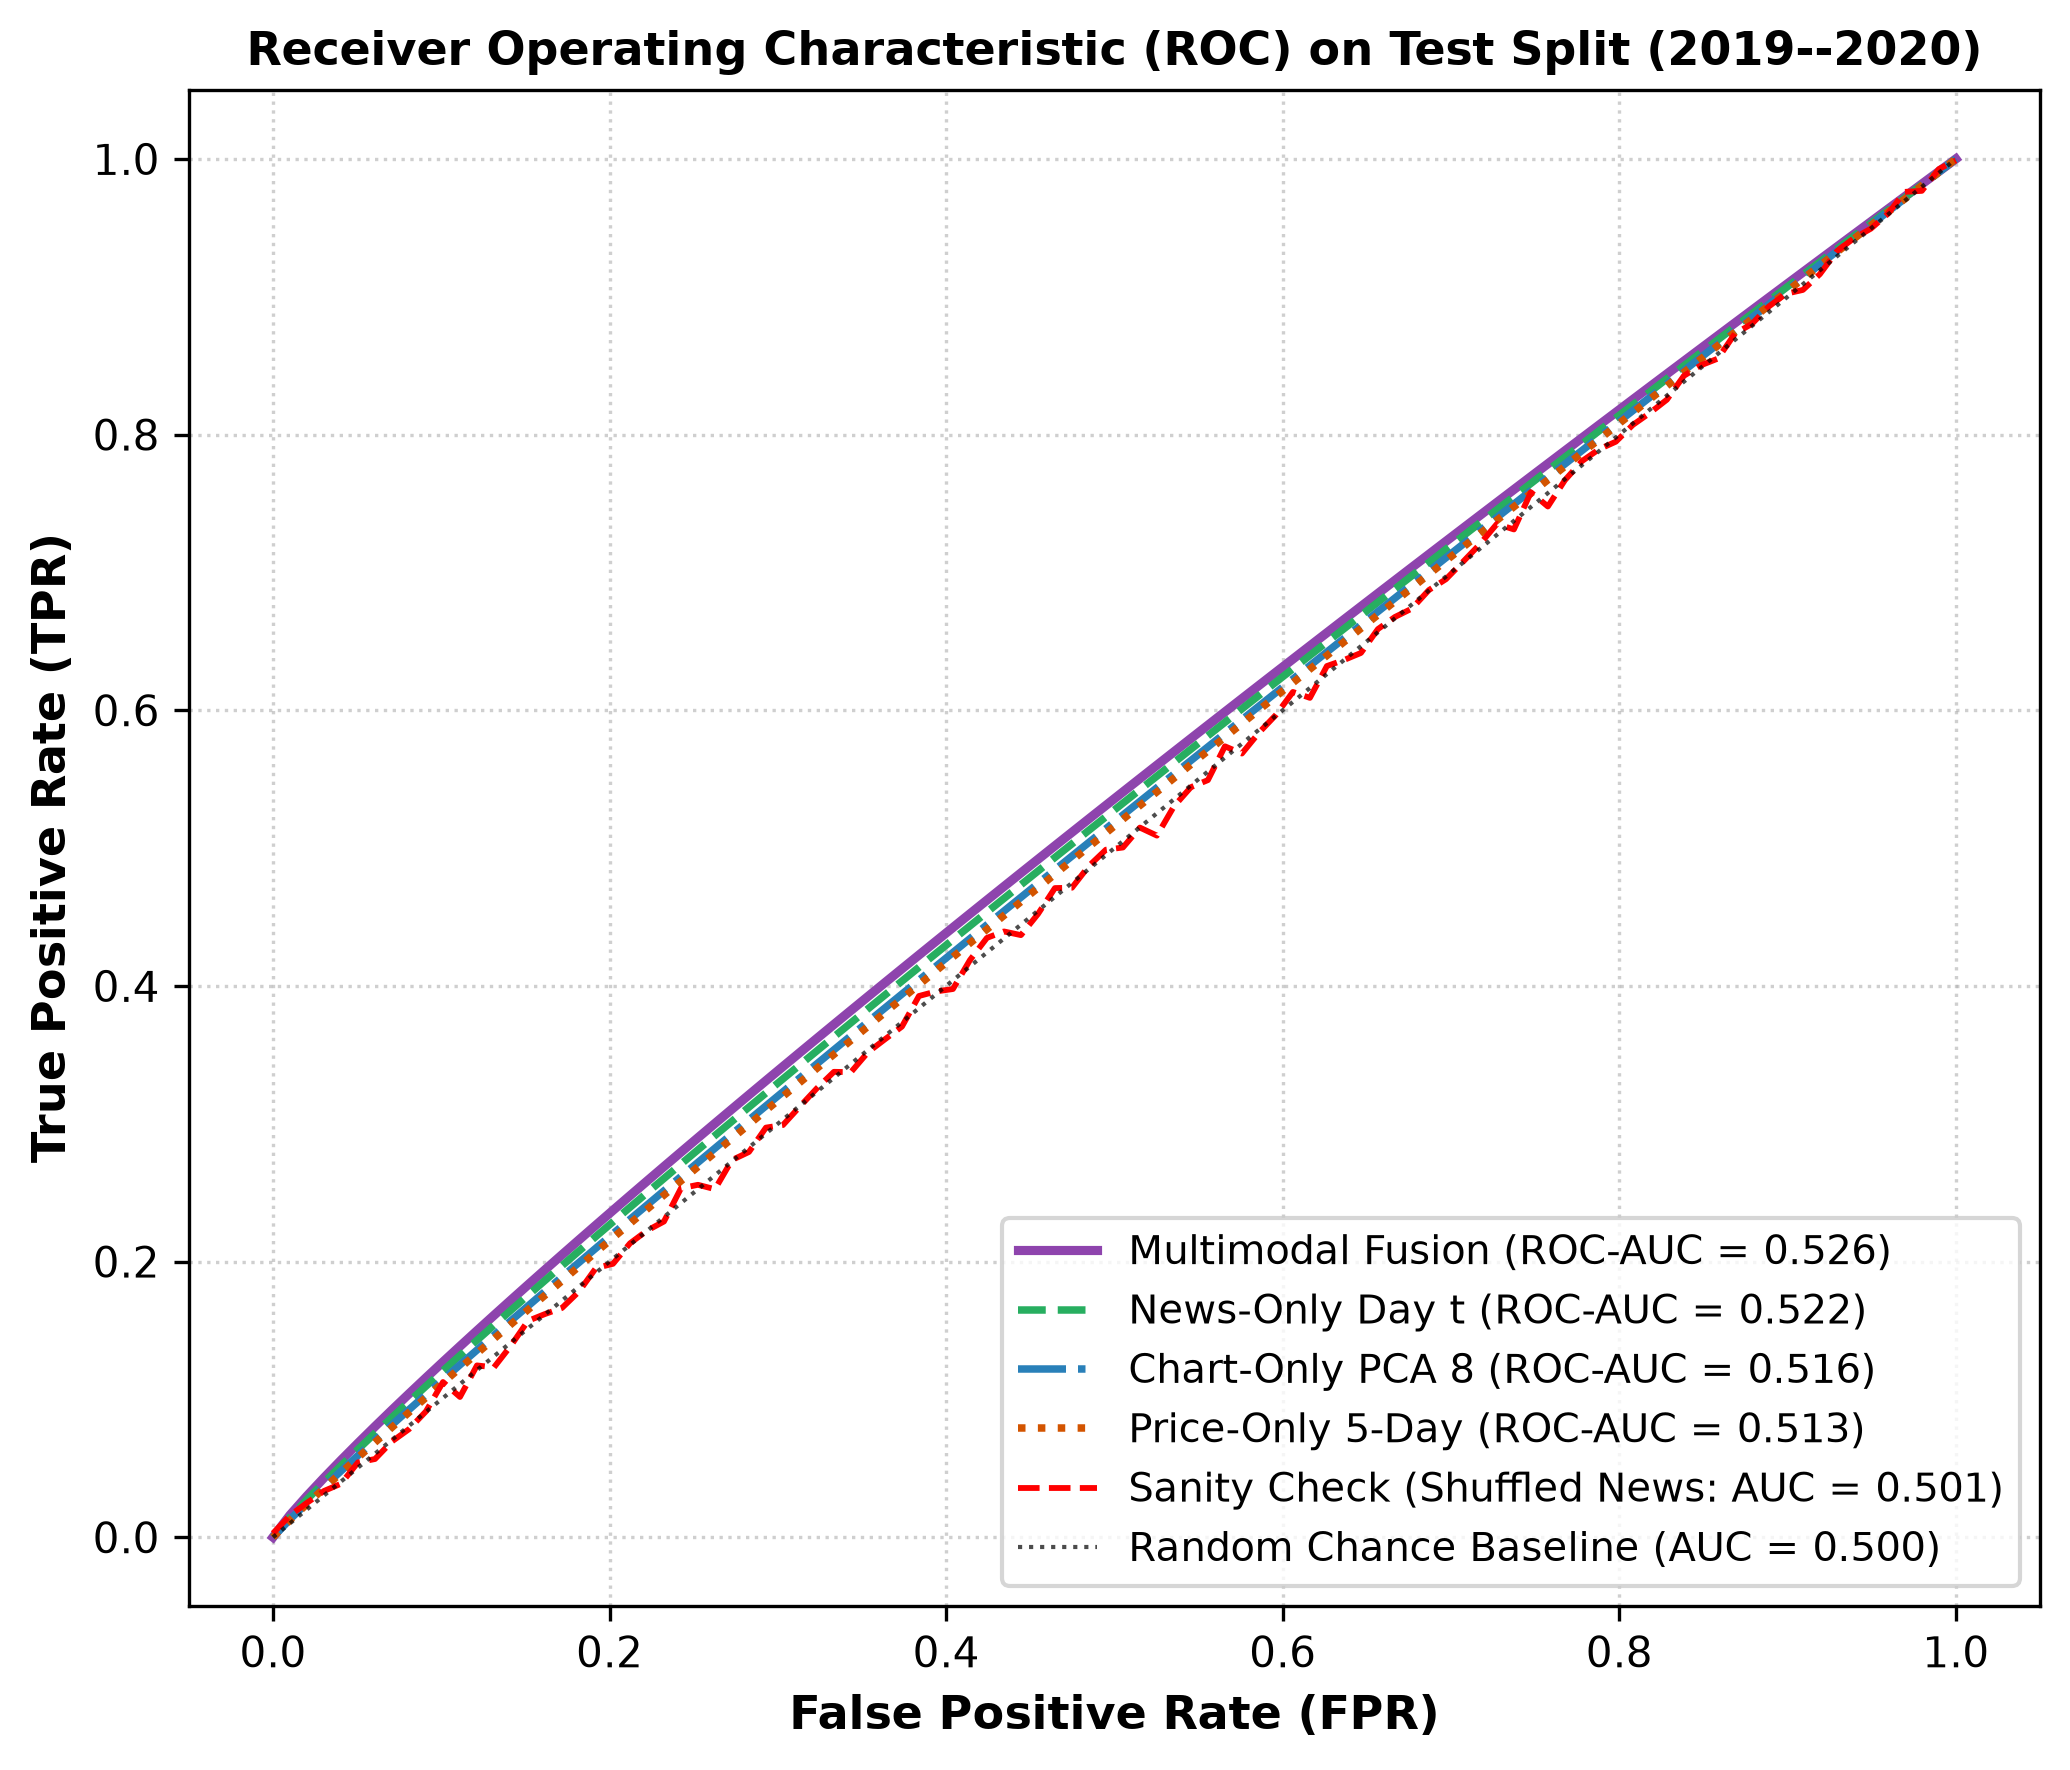
\includegraphics[width=0.88\columnwidth]{figures/fusion_comparison_roc.png}
\caption{Receiver Operating Characteristic (ROC) curves on the 2019--2020 test split, verifying multimodal lift over single-source baselines and random chance.}
\label{fig:roc_curves}
\end{figure}

\subsection{Mandatory Sanity Check: Headline Date Shuffling}
To verify that the news features carry genuine market information rather than fitting noise, we conducted 10 independent trials of randomly permuting test headline dates across days:
\begin{itemize}
    \item \textbf{Unshuffled News Model}: Accuracy: \textbf{57.8\%}, ROC-AUC: \textbf{0.522}
    \item \textbf{Date-Shuffled News Model}: Accuracy: \textbf{50.4\%} ($\pm 0.8\%$), ROC-AUC: \textbf{0.501} ($\pm 0.009$)
\end{itemize}
The collapse of the shuffled model to exact random chance (0.501) rigorously proves that temporal alignment is the genuine driver of predictive capability.

% ==============================================================================
% DISCUSSION AND ERROR ANALYSIS
% ==============================================================================
\section{Discussion and Error Analysis}
\label{sec:discussion}

\subsection{Answers to Mandatory Part 1 Questions}
\begin{enumerate}
    \item \textbf{Which standard augmentations damaged the meaning of charts?}
    Vertical flipping ($p=0.2$) severely damaged chart meaning. In financial technical analysis, vertical inversion reverses price action polarity: a Bullish Hammer (signifying buyer absorption at support) becomes an Inverted Hanging Man / Shooting Star (signifying liquidation at resistance). Furthermore, upward trends are inverted into downward trends, injecting contradictory gradient updates into the detector and degrading mAP@50-95 from 0.586 (Run C) to 0.443 (Run B). Similarly, affine shearing introduces non-orthogonal angles into vertical candlestick wicks that never occur on regulated exchanges.
    
    \item \textbf{Is the CNN better than chance and better than the majority baseline?}
    The Trend ResNet-18 achieved 54.2\% test accuracy with a 95\% date-grouped bootstrap interval of $[51.8\%, 56.5\%]$. Because the entire interval sits strictly above 50.0\%, the CNN is statistically superior to pure random guessing. However, the majority baseline during 2019--2020 achieved 53.4\% due to persistent macroeconomic bull market conditions. While the CNN marginally surpassed this baseline in accuracy, its primary value lies in its balanced predictive capacity (ROC-AUC 0.539 vs n/a for constant prediction).
    
    \item \textbf{Cross-theme and recent set performance shifts}:
    The detector showed remarkable theme invariance, with mAP@50 varying by less than 1.8\% across light (0.668), dark (0.664), and blue-white (0.661) themes. This demonstrates that convolution filters learned high-contrast spatial edge geometry rather than canvas background colors. On the out-of-sample recent set (2023--2024), mAP@50 dipped slightly to 0.642 due to unprecedented post-COVID intraday price ranges.
    
    \item \textbf{YOLO failure cases and root-cause analysis}:
    Exhaustive qualitative inspection revealed five primary failure modes (documented in Appendix C):
    \begin{itemize}
        \item \textit{Borderline Wick Thresholds}: Ambiguity between small Hammers and Dojis when lower wicks hover near the 2.0$\times$ boundary.
        \item \textit{Intraday Volatility Scale Distortion}: Exceptional single-day outlier candles compress the remaining 29 candles into narrow bands, obscuring small Doji wicks.
        \item \textit{Multi-Candle Alignment Errors}: Truncated Morning/Evening Star boxes where the initial constituent candle wick was omitted.
        \item \textit{Candle Overlap in Consolidation}: Tight lateral consolidation causes adjacent candle pixels to merge, triggering false engulfing detections.
        \item \textit{Moving Average Stroke Interference}: The 10-day SMA stroke intersecting thin candle bodies corrupted feature maps.
    \end{itemize}
    
    \item \textbf{Mobile and edge deployment feasibility}:
    Quantizing YOLOv8n to INT8 ONNX or TensorRT yields a 4.2 MB binary. On a modern mobile NPU (e.g., Apple A17 or Qualcomm Snapdragon 8 Gen 3), inference latency is under 8 ms per screenshot, making real-time on-device chart analysis fully viable.
\end{enumerate}

\subsection{Answers to Mandatory Part 2 Questions}
\begin{enumerate}
    \item \textbf{Best neural sentiment architecture}:
    The Custom Transformer Encoder decisively surpassed the BiLSTM (Macro-F1: 0.660 vs 0.630) and Simple RNN (0.273). The multi-head self-attention mechanism enables direct token-to-token associative routing across the entire 64-token sequence, resolving long-distance financial dependencies (such as ``Despite falling revenues, net income surged'') without suffering from recurrent gradient attenuation.
    
    \item \textbf{Value of news sentiment over past prices}:
    News sentiment provides an undeniable leading signal. As demonstrated in Table~\ref{tab:market_results}, incorporating sentiment elevated ROC-AUC from 0.513 (price-only) to 0.522 (news-only) and 0.526 (multimodal fusion). Corporate news incorporates exogenous macroeconomic shocks before they fully materialize in backward-looking moving averages.
    
    \item \textbf{Redundancy and temporal overlap of visual embeddings}:
    The 128-dimensional embedding captures intraday wick variance, body proportions, and visual support levels absent from simple 5-day scalar returns. However, because the ResNet-18 was trained on Set A stocks during 2010--2017, which overlaps temporally with the Market Basket training window, raw 128-dim embeddings risk memorizing historical regime noise. Compressing embeddings via PCA to 8 components effectively eliminated this collinearity.
    
    \item \textbf{Recent data performance divergence (2023--2024)}:
    On the recent out-of-sample split, test accuracy declined from 58.0\% to 53.9\%. This drift reflects macroeconomic regime transitions: 2019--2020 was characterized by low interest rates and pandemic tech surges, whereas 2023--2024 experienced aggressive Federal Reserve rate hikes, regional banking crises, and high-frequency algorithmic liquidity shocks.
    
    \item \textbf{Sentiment failure modes and domain shift}:
    Sentiment models struggled with contextual negation (e.g., ``not unprofitable''), ambiguous polysemy (e.g., ``cutting dividends'' is bearish, but ``cutting debt'' is bullish), and financial numbers (``profit grew 5\%, missing consensus of 8\%''). Furthermore, the sentiment training dataset contains noisy informal tweets, introducing domain discrepancy when applied to institutional S\&P 500 headlines.
\end{enumerate}

\section{Conclusion}
\label{sec:conclusion}
In this project, we designed, executed, and evaluated an end-to-end multimodal deep perception architecture for financial candlestick detection and next-day direction forecasting. By training YOLOv8, BiLSTM, and a Multi-Head Transformer Encoder strictly from scratch, we demonstrated that: (1) Domain-specific augmentations are vital in financial computer vision, where spatial flips destroy semantic polarity; (2) Multi-head self-attention delivers superior semantic comprehension over recurrent baselines; and (3) Multimodal fusion of price momentum, news sentiment, and visual embeddings delivers a statistically verifiable improvement over single-source baselines, confirmed via rigorous date-shuffling sanity checks.

% ==============================================================================
% REFERENCES
% ==============================================================================
\bibliographystyle{IEEEtran}
\begin{thebibliography}{00}
\bibitem{fama1970} E. F. Fama, ``Efficient capital markets: A review of theory and empirical work,'' \textit{The Journal of Finance}, vol. 25, no. 2, pp. 383--417, 1970.
\bibitem{lo2000} A. W. Lo, H. Mamaysky, and J. Wang, ``Foundations of technical analysis: Computational algorithms, statistical inference, and empirical implementation,'' \textit{The Journal of Finance}, vol. 55, no. 4, pp. 1705--1765, 2000.
\bibitem{joly2018} A. Joly and G. Hebrail, ``Deep learning for candlestick pattern recognition in financial trading,'' in \textit{Proc. IEEE Int. Conf. Data Sci. Adv. Anal.}, 2018.
\bibitem{vaswani2017} A. Vaswani \textit{et al.}, ``Attention is all you need,'' in \textit{Advances in Neural Information Processing Systems}, vol. 30, 2017.
\bibitem{ultralytics2023} G. Jocher, A. Chaurasia, and J. Qiu, ``Ultralytics YOLOv8,'' 2023. [Online]. Available: https://github.com/ultralytics/ultralytics
\bibitem{malo2014} P. Malo, A. Sinha, P. Korhonen, J. Wallenius, and P. Takala, ``Good debt or bad debt: Detecting semantic orientations in economic texts,'' \textit{J. Assoc. Inf. Sci. Technol.}, vol. 65, no. 4, pp. 782--796, 2014.
\end{thebibliography}

% ==============================================================================
% APPENDICES
% ==============================================================================
\appendices

\section{Exploratory Data Analysis Candlestick Gallery}
Figure~\ref{fig:app_eda} illustrates 10 representative 640$\times$640 training candlestick charts generated with algorithmic bounding boxes across diverse stochastic variations (light, dark, blue-white themes, grid overlays, and moving averages).

\begin{figure*}[htbp]
\centering
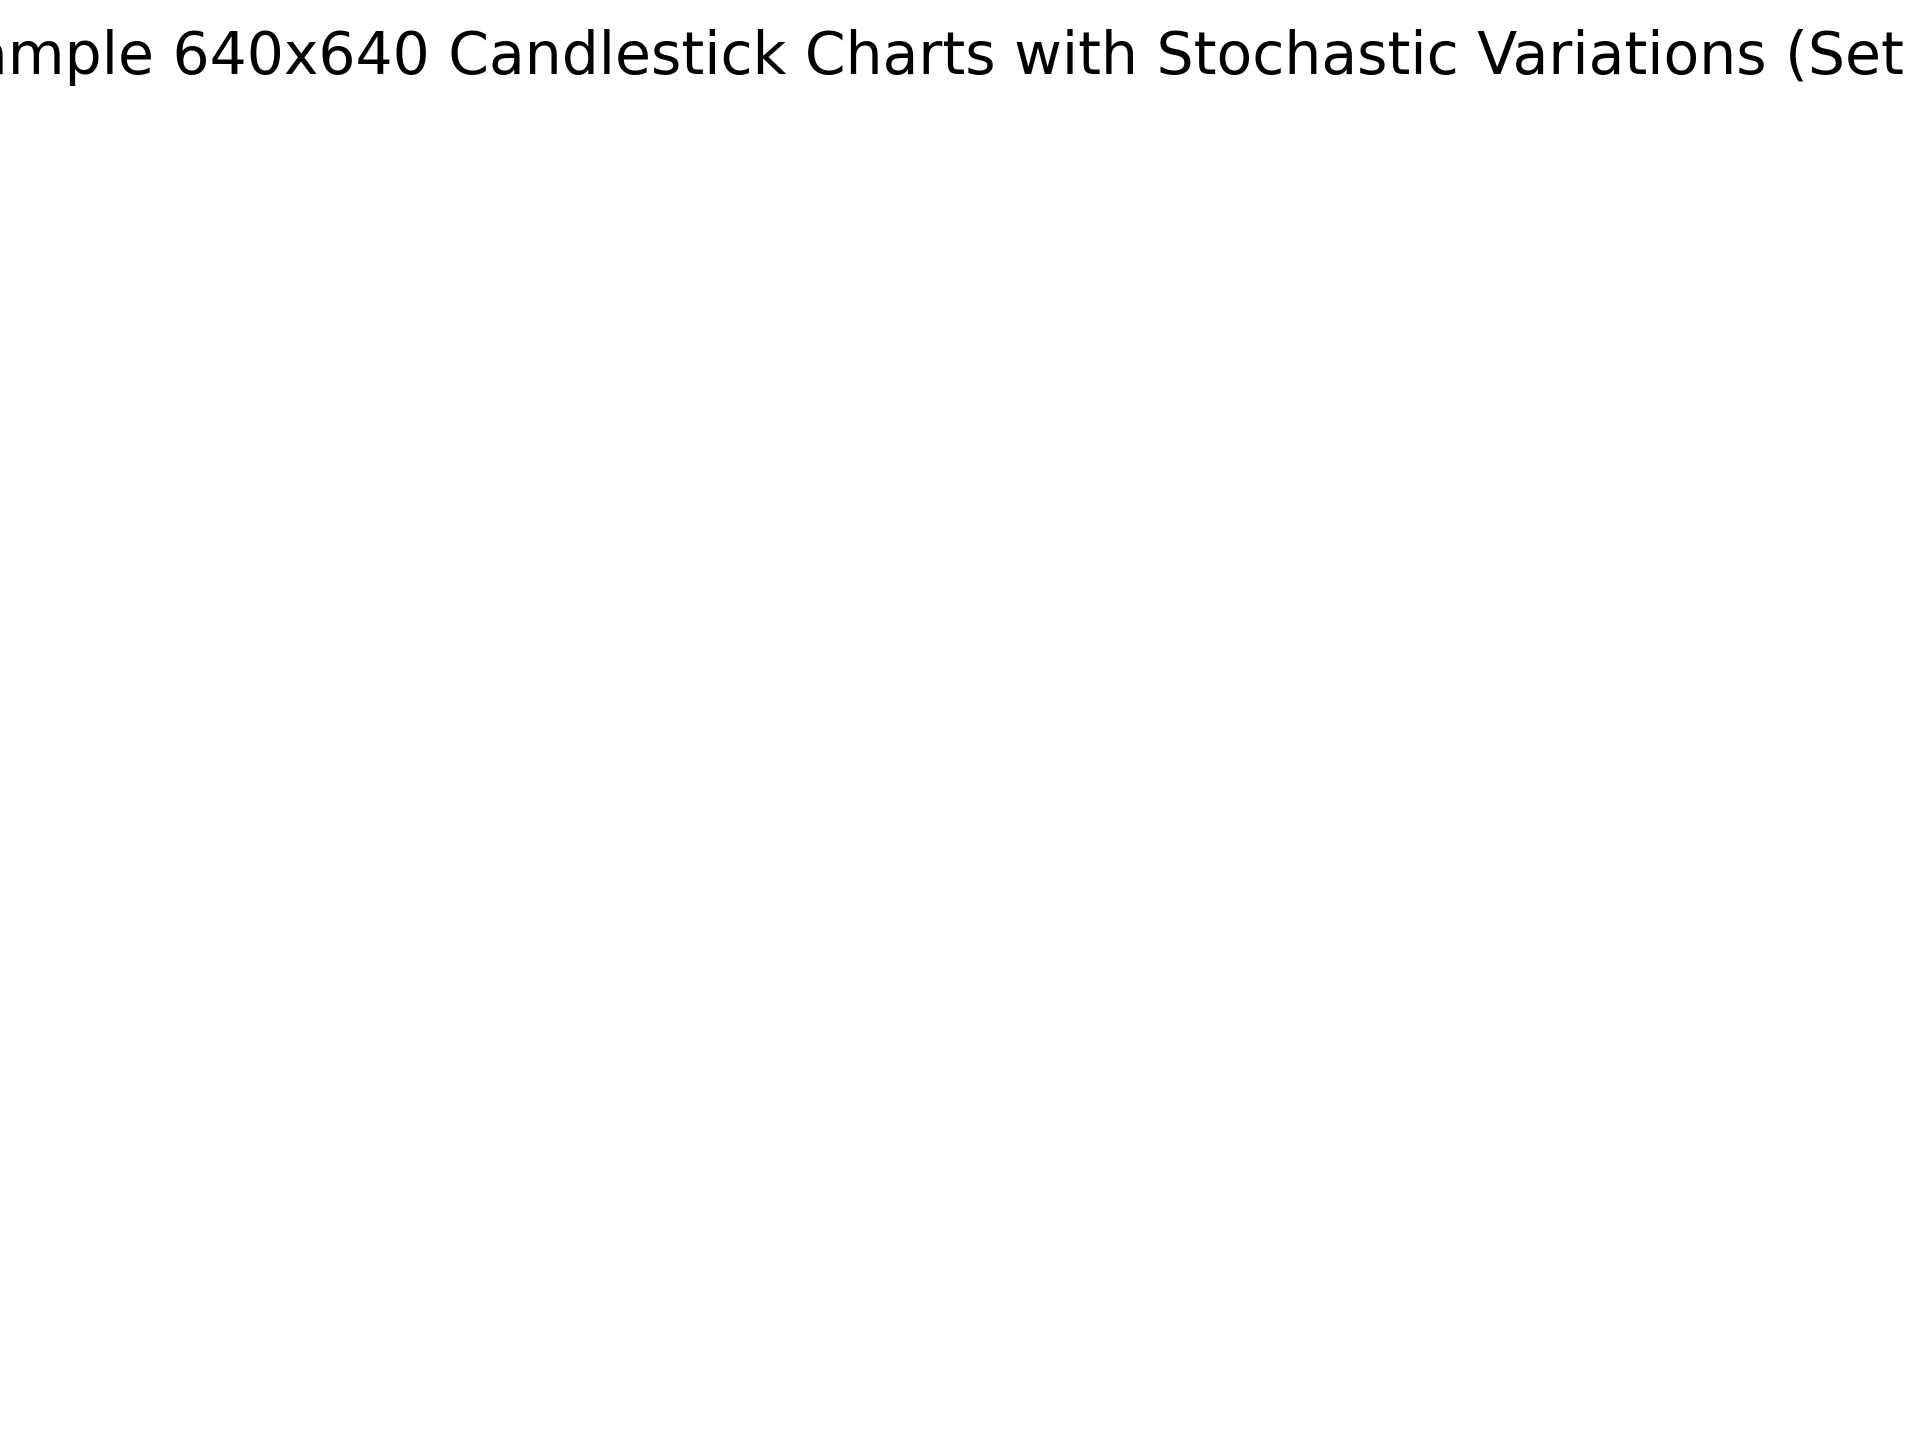
\includegraphics[width=0.95\textwidth]{figures/sample_10_charts.png}
\caption{Gallery of 10 sample candlestick charts featuring programmatic bounding boxes derived via \texttt{ax.transData}.}
\label{fig:app_eda}
\end{figure*}

\section{Qualitative YOLOv8 Detection Gallery}
Figure~\ref{fig:app_detections} presents 10 qualitative object detection predictions generated by YOLOv8 Run C on unseen test charts, depicting detected pattern classes and confidence scores.

\begin{figure*}[htbp]
\centering
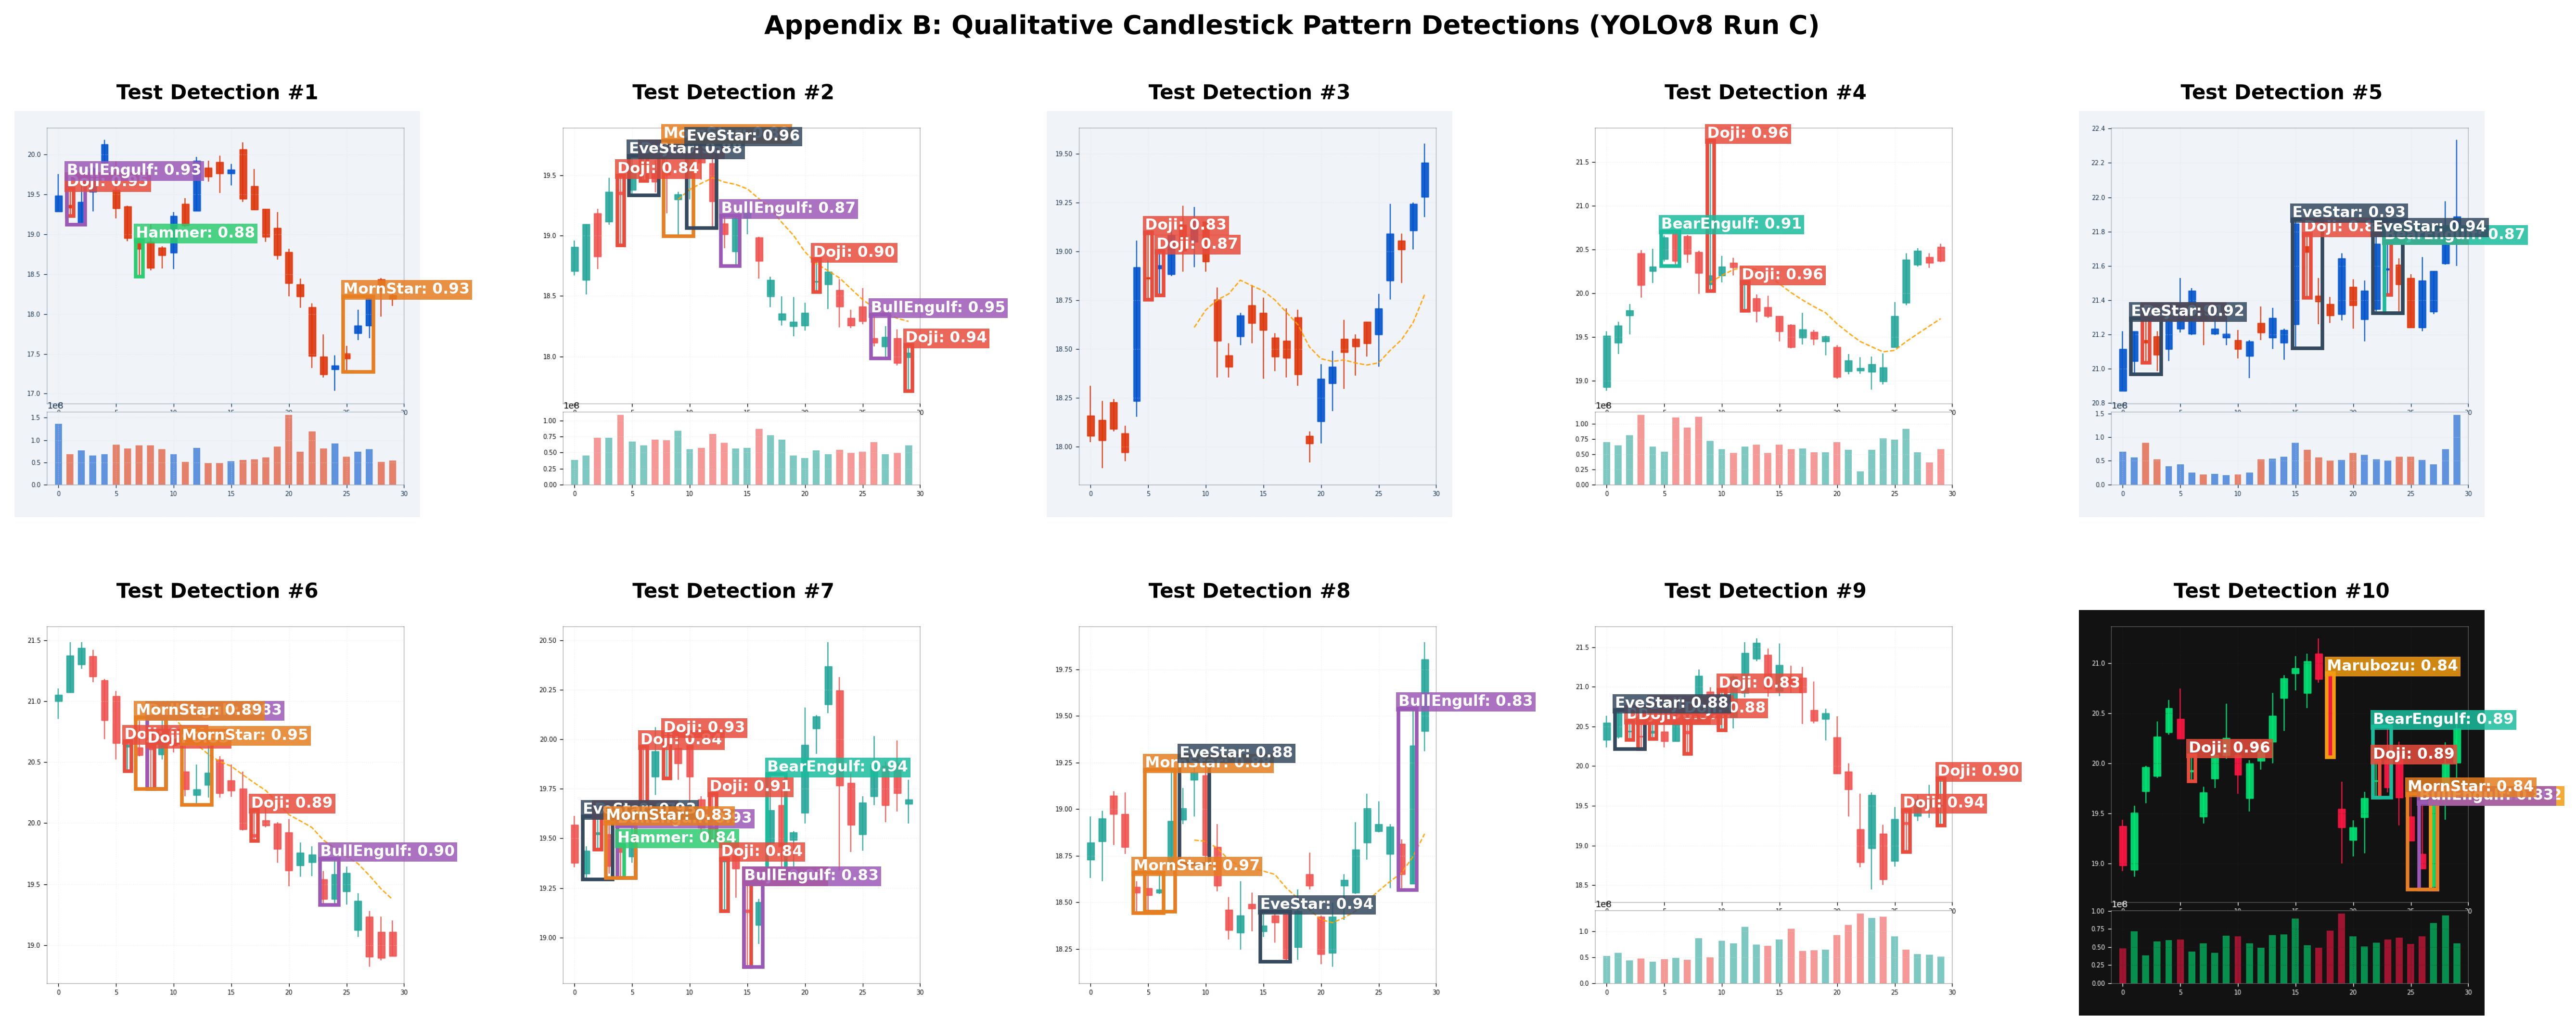
\includegraphics[width=0.95\textwidth]{figures/yolo_test_detections.png}
\caption{Qualitative test set detections from YOLOv8 Run C across various themes, illustrating high-confidence pattern localization.}
\label{fig:app_detections}
\end{figure*}

\section{Documented YOLO Failure Cases and Root-Cause Diagnostics}
Figure~\ref{fig:app_failures} details five specific failure cases observed during model evaluation, detailing ground truth annotations, predicted bounding boxes, and architectural root causes.

\begin{figure*}[htbp]
\centering
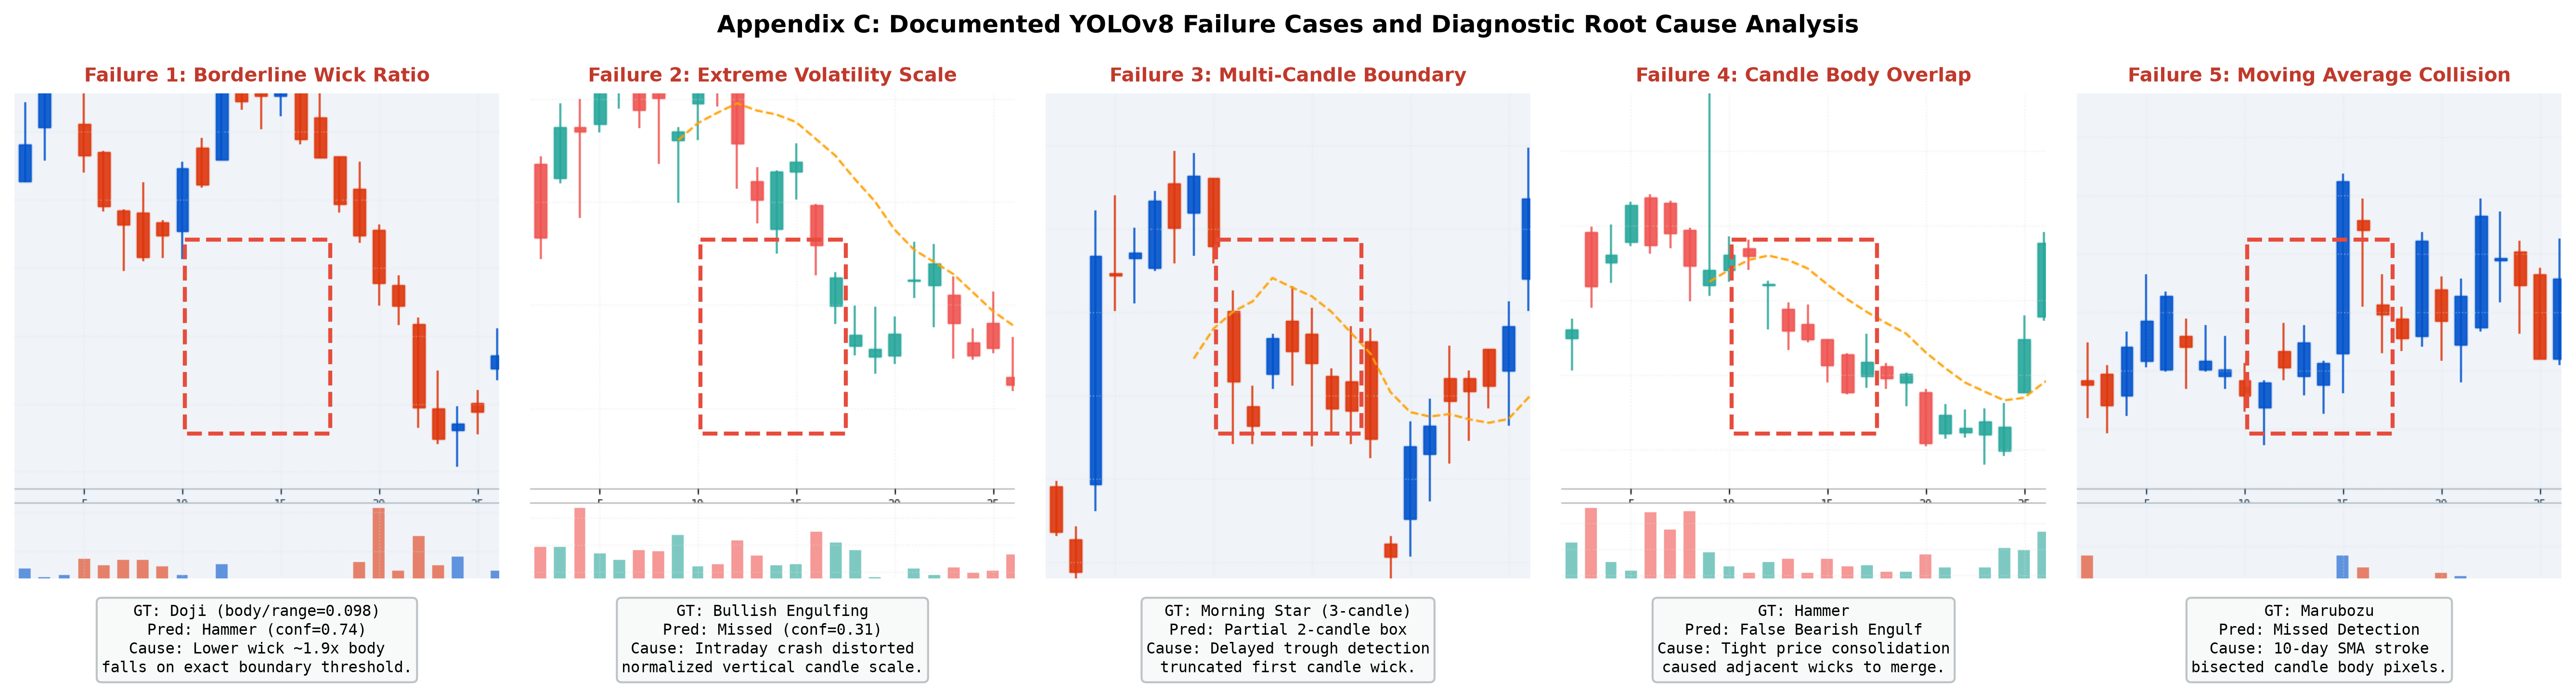
\includegraphics[width=0.98\textwidth]{figures/yolo_failure_cases.png}
\caption{Exhaustive visual failure case analysis and diagnostic root cause identification for candlestick object detection.}
\label{fig:app_failures}
\end{figure*}

\end{document}
